% Exemplo de dissertação do INF-UFG com texto em portugues formatado com LaTeX
\documentclass[relatorio, nocolorlinks]{inf-ufg}
% Opções da classe inf-ufg (ao usar mais de uma, separe por vírgulas)
%   [tese]         -> Tese de doutorado.
%   [dissertacao]  -> Dissertação de mestrado (padrão).
%   [monografia]   -> Monografia de especialização.
%   [relatorio]    -> Relatório final de graduação.
%   [abnt]         -> Usa o estilo "abnt-alf" de citação bibliográfica.
%   [nocolorlinks] -> Os links de navegação no texto ficam na cor preta.
%                     Use esta opção para gerar o arquivo para impressão
%                     da versão final do seu texto!!!

%----------------------------------------------------- INICIO DO DOCUMENTO %
\usepackage{caption}
\usepackage{amsmath}
\usepackage{pdfpages}
\begin{document}

%------------------------------------------ AUTOR, TÍTULO E DATA DE DEFESA %
\autor{Bryan Lincoln Marques de Oliveira} % (José da Silva)
\autorR{Oliveira, Bryan Lincoln Marques de} % (da Silva, José)

\titulo{Motivação intrínseca para aprendizado de manipulação robótica com recompensas esparsas}
% \subtitulo{ Subtítulo do Trabalho }

\cidade{Goiânia} % Nome da cidade em foi desenvolvido o trabalho
\dia{12} %
\mes{dezembro} % Data da apresentação/defesa do trabalho
\ano{2019} % Formato numérico: \dia{01}, \mes{01} e \ano{2009}

%-------------------------------------------------------------- ORIENTADOR %
\orientadora{Dra. Telma Woerle de Lima Soares}
\orientadoraR{Lima, Telma Woerle de}
% Use os comandos a seguir se for Orientadora e nao Orientador.
%\orientadora{\textless Nome da Orientadora\textgreater}
%\orientadoraR{\textless Nome Reverso da Orientadora\textgreater}

%\coorientador{\textless Nome do Co-orientador\textgreater}
%\coorientadorR{\textless Nome Reverso do Co-orientador\textgreater}
% Use os comandos a seguir se for Co-orientadora e nao Coorientador.
%\coorientadora{\textless Nome da Co-orientadora\textgreater}
%\coorientadoraR{\textless Nome Reverso da Co-orientadora\textgreater}

%-------------------------------------------------- INSTITUIÇÃO E PROGRAMA %
\universidade{Universidade Federal de Goiás} % {Universidade Federal de Goiás}
\uni{UFG}         % UFG
\unidade{Instituto de Informática} %Instituto de Informática
%\departamento{\textless Nome do Departamento\textgreater} %Unidades com mais de um depto.

%\universidadeco{\textless Nome da Universidade do Co-orientador\textgreater}
%\unico{\textless Sigla da Universidade do Co-orientador\textgreater}
%\unidadeco{\textless Nome da Unidade Acadêmica do Co-orientador\textgreater}

\programa{Ciências da Computação} % Computação
\concentracao{Ciências da Computação, Inteligência Artificial}

%-------------------------------------------------- ELEMENTOS PRÉ-TEXTUAIS %
\capa    % Gera o modelo da capa externa do trabalho
%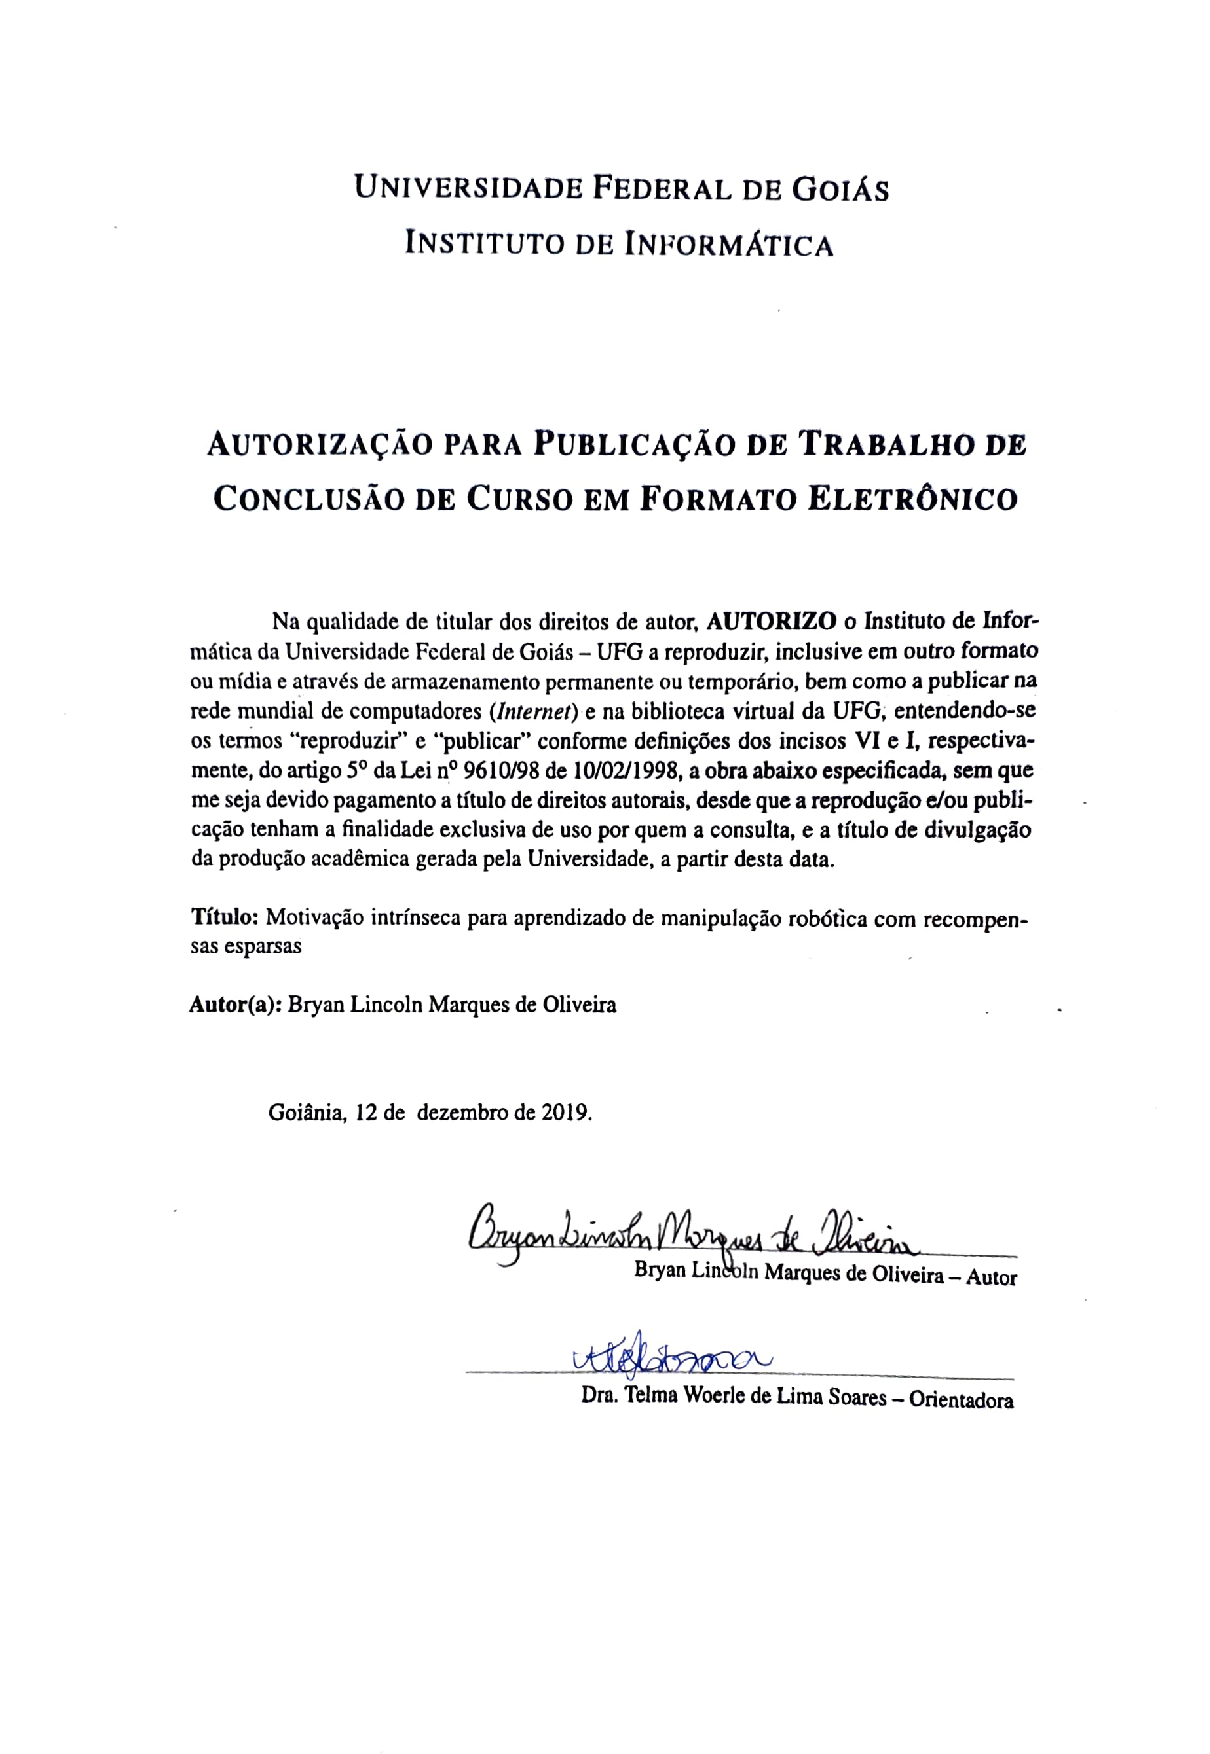
\includepdf[pages=1, offset=0 -75]{./pre/autorizacao}
%\publica % Gera a autorização para publicação em formato eletrônico
\rosto   % Primeira folha interna do trabalho

\begin{aprovacao}
\banca{Dr. Anderson da Silva Soares}{Instituto de Informática -- UFG}
\end{aprovacao}
%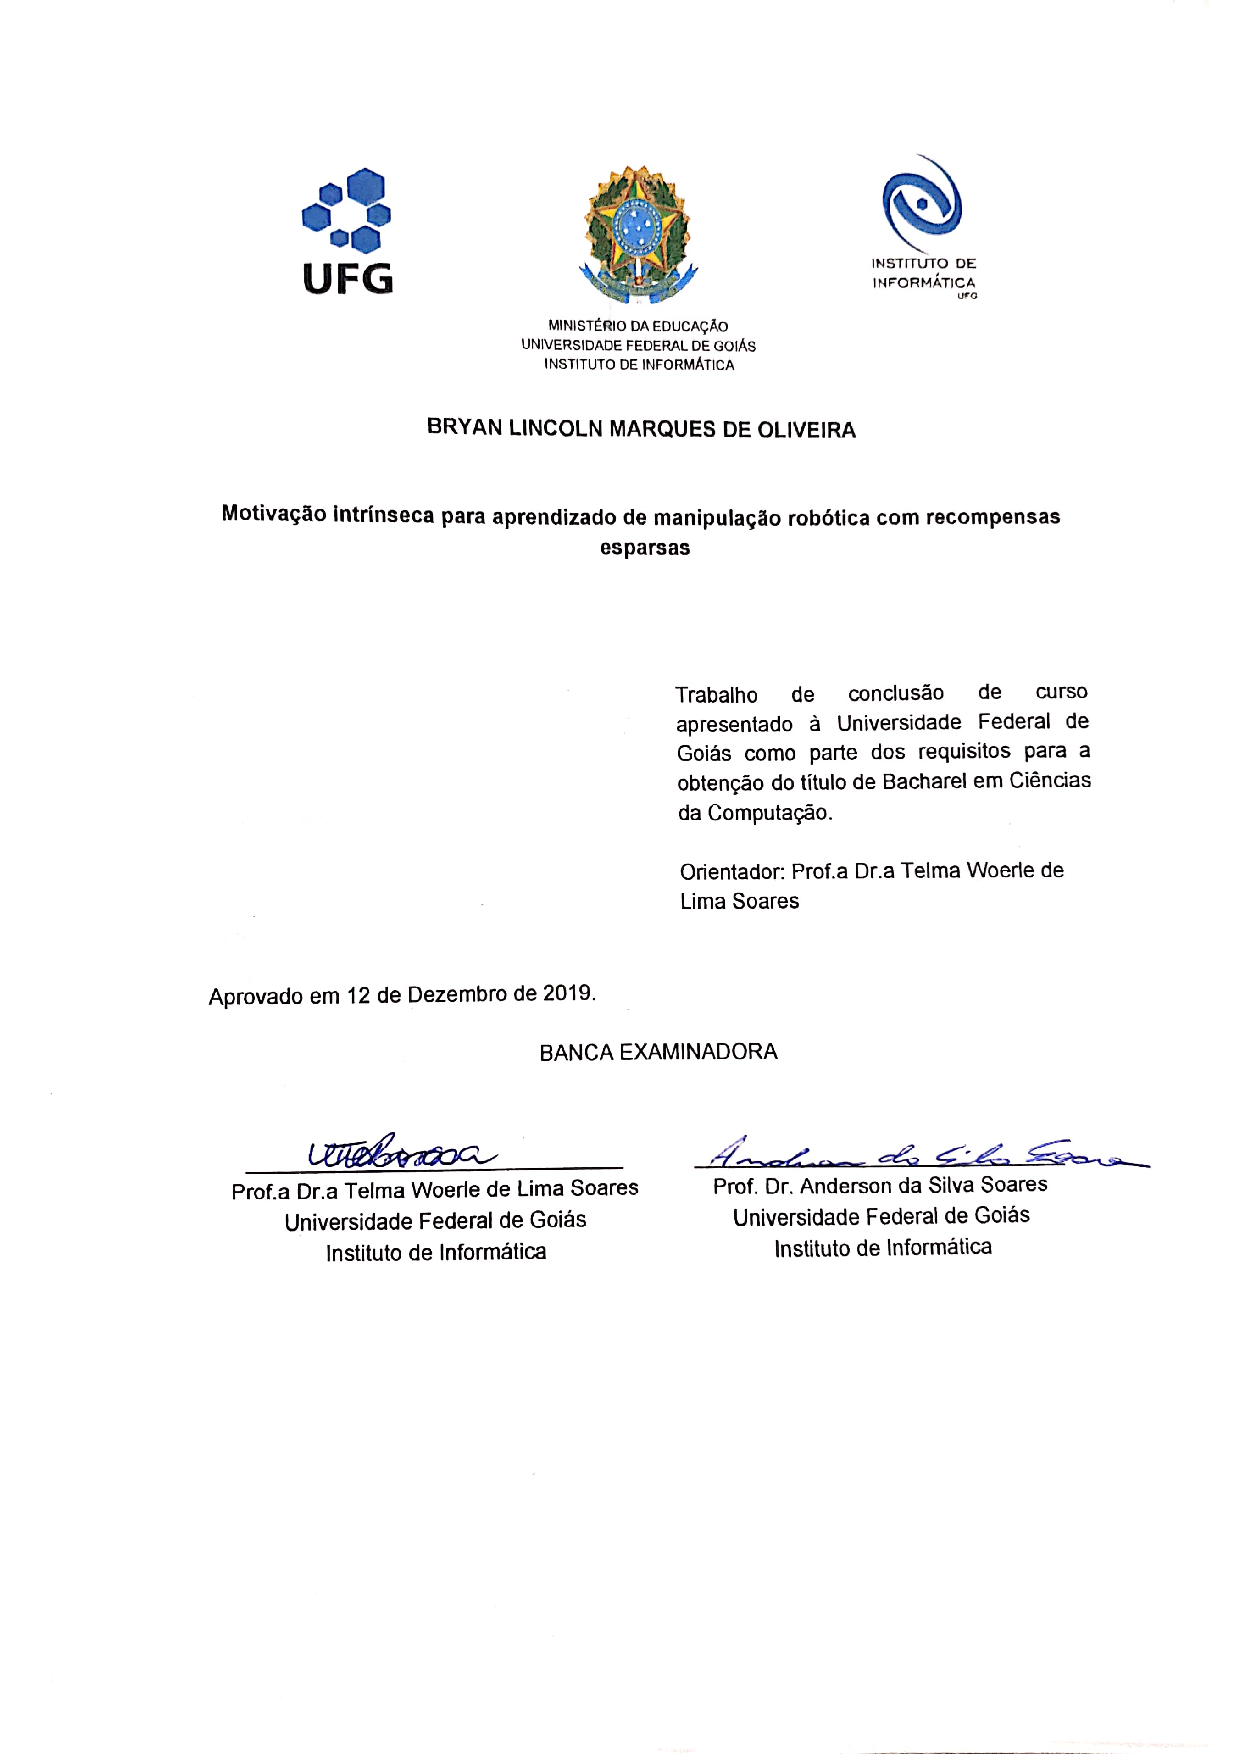
\includepdf[pages=1, offset=-10 -75]{./pre/aprovacao}
\direitos{
Graduando em Ciências da Computação pelo Instituto de Informática na Universidade Federal de Goiás. Durante a graduação foi monitor das disciplinas de Programação de Computadores e Matemática Discreta. Atualmente estuda e desenvolve na área de Aprendizado por Reforço pelo laboratório Deep Learning Brasil.
}
\begin{dedicatoria}
A todos aqueles que contribuíram direta ou indiretamente para meu crescimento pessoal e profissional.
\end{dedicatoria}
\begin{agradecimentos}
Agradeço à minha família por todo o apoio durante minha jornada nesta graduação. Agradeço também à minha incrível namorada, Luana, por toda a motivação e companheirismo que permitiram visar objetivos ainda maiores. Aos meus amigos, pelos momentos de descontração e discussões construtivas. Ao Núcleo de Robótica Pequi Mecânico, pelas amizades, conhecimento técnico e ajuda no desenvolvimento de habilidades interpessoais. Agradeço também aos meus professores, pela excelência e qualidade técnica que me fizeram ter amor pela área. Em especial, agradeço à Profa. Dra. Telma Woerle de Lima Soares pela orientação neste trabalho e ao Prof. Dr. Anderson da Silva Soares pelo suporte fornecido. Agradeço também ao laboratório Deep Learning Brasil e aos membros do grupo de Aprendizado por Reforço, em especial ao MSc. Luckeciano Carvalho Melo, pelos valiosos \textit{insights} e experiência compartilhada. Por fim, agradeço à COPEL e ao laboratório Deep Learning Brasil pelo auxílio financeiro que possibilitou a dedicação e a operacionalização do estudo.
\end{agradecimentos}
\epigrafe{If a machine is expected to be infallible, it cannot also be intelligent.}
{Alan Mathison Turing}
{B. J. Copeland (2004). “The Essential Turing”, p.394, Oxford U. Press}

\chaves{Inteligência Artificial; Aprendizado por Reforço; Redes Neurais; Robótica.}

\begin{resumo} 
Algoritmos de Aprendizado de Máquina têm se tornado cada vez mais eficientes em resolver problemas complexos do mundo real. Em especial, algoritmos de Aprendizado por Reforço são capazes de aprender comportamentos aplicáveis à robótica que podem substituir ou trabalhar em conjunto de modelos de controle clássico, aumentando assim sua robustez, aplicabilidade e viabilidade. No entanto, resta a dificuldade de se elaborar funções de recompensa que representem, para um agente de aprendizado por reforço, a tarefa que este deve executar. Pesquisas recentes nessa área propõem técnicas como curiosidade e motivação intrínseca como alternativa ao uso de recompensas extrínsecas do ambiente, se mostrando eficientes em guiar o agente a exploração satisfatória em ambientes de jogos como \textit{VizDoom} e \textit{Super Mario Bros}. Neste trabalho é analisado o impacto da técnica de motivação intrínseca no treinamento de agentes em ambientes de simulação robótica, assim como implicações gerais que a mesma tem sobre aspectos como generalização e eficiência de exploração e amostragem nos mesmos. Como resultado, são encontradas evidências de que a motivação intrínseca influencia positivamente na descoberta de comportamentos complexos por parte dos agentes, mantendo uma tendência para altos níveis de exploração mesmo após sua convergência.

\end{resumo}


\keys{Artificial Intelligence; Reinforcement Learning; Neural Networks; Robotics.}

\begin{abstract}{Intrinsic motivation for robotic manipulation learning with sparse rewards}
Machine Learning Algorithms have become increasingly efficient at solving complex real-world problems. In particular, Reinforcement Learning algorithms are capable of learning behaviors applicable to robotics that can replace or work together with classical control models, thereby increasing their robustness, applicability and viability. However, it remains difficult to design reward functions that represent, for a reinforcement learning agent, the task it must perform. Recent research in this area proposes techniques such as curiosity and intrinsic motivation as an alternative to the use of extrinsic environmental rewards, proving to be efficient in guiding the agent to satisfactory exploration in game environments such as \textit{VizDoom} and \textit{Super Mario Bros}. This paper analyzes the impact of the intrinsic motivation technique on agent training in robotic simulation environments, as well as its general implications for aspects such as generalization, exploration and sampling efficiency. As a result, evidence is found that intrinsic motivation positively influences the agents' discovery of complex behaviors, maintaining a tendency for high levels of exploitation even after it's convergence.

\end{abstract}

\tabelas[figtabalg]
%Opções:
%nada [] -> Gera apenas o sumário
%fig     -> Gera o sumário e a lista de figuras
%tab     -> Sumário e lista de tabelas
%alg     -> Sumário e lista de algoritmos
%cod     -> Sumário e lista de códigos de programas
%
% Pode-se usar qualquer combinação dessas opções.
% Por exemplo:
%  figtab       -> Sumário e listas de figuras e tabelas
%  figtabcod    -> Sumário e listas de figuras, tabelas e
%                  códigos de programas
%  figtabalg    -> Sumário e listas de figuras, tabelas e algoritmos
%  figtabalgcod -> Sumário e listas de figuras, tabelas, algoritmos e
%                  códigos de programas

%--------------------------------------------------------------- CAPÍTULOS %

\chapter{Introdução}
\label{cap:intro}

Desde os últimos anos, algoritmos de Inteligência Artificial (IA) vêm sendo aplicados com grande sucesso em diversos setores da indústria e da sociedade. Suas soluções resolvem problemas que variam desde a detecção, classificação e acompanhamento de doenças \cite{dldiabetic, dlalzheimer} a segmentação de ruas, carros e pedestres para navegação autônoma \cite{pan2017agile, autonomousvehicle}. Aplicações como essas não só permitem a solução de problemas antes inviáveis de se atacar como também permitem a substituição de processos caros e demorados.

Junto dos avanços da IA, avanços na robótica permitiram sua aplicação em tarefas de alta precisão que variam desde impressões 3D a execução de acrobacias \cite{atlaspaper}. Além disso, manipuladores robóticos têm se tornado quase omnipresentes em linhas de produção de indústrias em todo o mundo \cite{automatedassembly}. Em contrapartida, as técnicas de controle mais utilizadas nessas tarefas envolvem o desenvolvimento de modelos matemáticos complexos que devem ser precisamente construídos. Esses modelos levam em consideração, por exemplo, as características físicas do equipamento (e.g. distribuição de massa e torque máximo dos atuadores) e do ambiente (e.g. atrito com o chão, gravidade e rotação da Terra) \cite{coriolis}. A criação desses modelos pode se mostrar uma tarefa consideravelmente difícil e cara para ser executada em larga escala, principalmente quando o equipamento utilizado é formado por numerosas partes móveis e seu ambiente de trabalho é irregular.

Boa parte dos maiores desafios de implementação de robôs com comportamentos complexos são desafios de \textit{software} \cite{dlrobotics}. Especialistas em controle e automação dedicam tempo considerável programando as ações dos atuadores robóticos para que estes executem suas tarefas de forma satisfatória. Outro problema é a falta de generalização de um comportamento entre diferentes equipamentos. Um comportamento programado para um hardware e estrutura específicos é dificilmente portado para outro sem diversos ajustes finos.

Pesquisas recentes em técnicas de IA aplicada a robótica, em especial de aprendizado por reforço, revelaram-se eficazes em substituir a necessidade de comportamentos estritamente programados para execução de tarefas \cite{openaihand, rlindustrial}. Essas técnicas são capazes de aprender comportamentos do zero em simulação de forma que seja possível portá-los para o mundo real mantendo sua robustez a adversidades do ambiente \cite{Tobin_2017}. Além disso, técnicas de aprendizado que trabalham em conjunto de técnicas clássicas a fim de permitir o porte de um comportamento de um equipamento para outro também foram desenvolvidas \cite{rlforcontrol}, permitindo a adaptação do agente para diferentes condições físicas.

Agentes de aprendizado por reforço trabalham com base nos sinais de retorno dados pelo ambiente em que são inseridos. Um problema que surge, com isso, é a necessidade de que os sinais, ou recompensas, guiem o aprendizado para o objetivo esperado. Mesmo sendo um processo menos trabalhoso que a construção de modelos de cinemática inversa, comportamentos complexos como locomoção e manipulação de objetos requerem a modelagem de sinais de recompensa que levam em consideração diversos fatores que podem ser difíceis de se descobrir e balancear \cite{dexterity, ng, deepLoco}. Além disso, frequentemente agentes de aprendizado por reforço encontram problemas no sinal de recompensa modelado que os permitem maximizar seu valor acumulado sem executar a tarefa originalmente proposta \cite{rewardhacking, rewardfaulty}.

Naturalmente, o sinal de recompensa mais simples em tarefas do mundo real diz apenas se um objetivo foi alcançado ou não, ou seja, a recompensa é esparsa em relação as ações tomadas pelo algoritmo. Algoritmos convencionais de aprendizado por reforço tendem a ter dificuldades em aprender em configurações desse tipo \cite{hindsight}. Como alternativa, as noções da psicologia de motivação intrínseca \cite{intrinsicryan} e curiosidade \cite{CuriosityandMotivation} foram aplicadas ao aprendizado por reforço com o objetivo de incentivar a exploração dos agentes em busca de recompensas extrínsecas \cite{curiositylarge, pathak}.

Este trabalho tem como objetivo a aplicação e a avaliação dos conceitos e técnicas de motivação intrínseca para exploração em ambientes de manipulação robótica com recompensa esparsa, dado o sucesso da aplicação destas técnicas em jogos de \textit{Atari}, \textit{Mario} e \textit{VizDoom} \cite{curiositylarge, pathak}. Para isso, este trabalho está organizado da seguinte maneira: no Capítulo \ref{cap:fundamentacao} é apresentada a fundamentação teórica dos conceitos utilizados para a execução dos experimentos; no Capítulo \ref{cap:metodologia} é descrito o ambiente utilizado, o algoritmo proposto e a definição dos testes; no Capítulo \ref{cap:resultados} são apresentados os resultados e no Capítulo \ref{cap:conclusao} são apresentadas as conclusões deste trabalho.
\chapter{Fundamentação Teórica}
\label{cap:fundamentacao}
Neste capítulo serão apresentados os conceitos teóricos que são base para este trabalho. Primeiramente será introduzido o funcionamento básico das redes neurais e das redes neurais profundas. Em seguida, será apresentado o conceito de aprendizado de máquina, onde serão definidas as técnicas de aprendizado supervisionado, não supervisionado e por reforço. Depois, será definido em mais detalhes a motivação e os tipos de aprendizado por reforço, assim como a Estimativa de Vantagem Generalizada e o algoritmo \textit{Proximal Policy Optimization} que são utilizados como ferramenta neste trabalho. Por fim, serão apresentadas os principais problemas relacionados a ambientes com recompensa esparsa no contexto de aprendizado por reforço e será introduzida a técnica de exploração por curiosidade e motivação intrínseca.

%% - - - - - - - - - - - - - - - - - - - - - - - - - - - - - - - - - - -

\section{Redes Neurais}
\label{sec:redesneurais}

Redes Neurais Artificiais (RNAs) são técnicas computacionais para modelagem matemática inspiradas pelo sistema nervoso central de organismos inteligentes. RNAs são tipicamente utilizadas como aproximadoras de funções universais e possuem estruturas que fazem um paralelo entre mecanismos biológicos como neurônios, sinapses e diferentes organizações estruturais (topologias) \cite{Russel}. 

% \subsection{Neurônio}

\begin{figure}[ht]
 \centering
  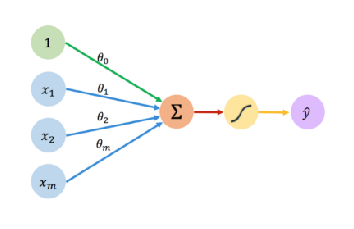
\includegraphics[width=0.5\textwidth]{./fig/Neuron}
  \caption{Diagrama do funcionamento de um neurônio.}
 \label{fig:neuron}
\end{figure}

A unidade mais básica de processamento de uma rede neural é o neurônio, que recebe um ou mais valores $x_i$ como entrada, multiplica-os pelo peso sináptico correspondente $\theta_i$ e adiciona sua soma a um valor $b$ conhecido como \textit{bias} \cite{Goodfellow2016}. O valor final é alimentado a uma função de ativação que induz a não-linearidade da função aproximada pelo sistema. Este processo é demonstrado na Figura \ref{fig:neuron}.

De uma forma mais didática, o parâmetro $\theta_i$ define quanto de um sinal $x_i$ deverá ser considerado no processamento do neurônio e $b$ permite que o neurônio ajuste o sinal de saída de uma forma independente dos sinais de entrada. A função de ativação permite o neurônio representar funções mais complexas que funções lineares \cite{Luckeciano}. A Equação \ref{eqn:neuron} descreve o processamento de um neurônio.

\begin{equation}
\label{eqn:neuron}
\hat{y} = \sigma(w^Tx+b)
\end{equation}

Dentre as funções de ativação mais utilizadas na prática estão a \textit{Rectified Linear Unit} (ReLU), a tangente hiperbólica (TanH) e a função sigmóide, utilizada na Equação \ref{eqn:neuron}. Cada função de ativação possui um comportamento específico, que pode ser observado na Figura \ref{fig:activationfunctions}.

\begin{figure}[ht]
 \centering
  \subfigure[ReLU.]
   {
    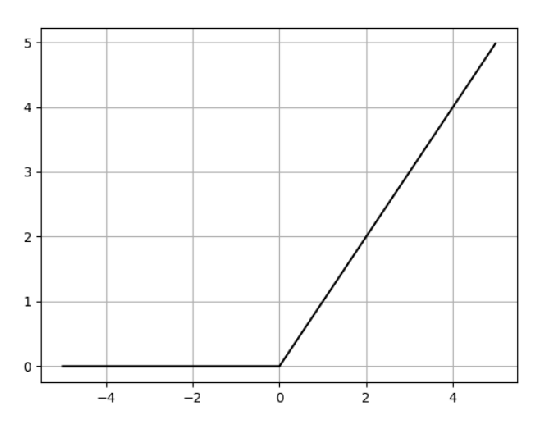
\includegraphics[width=0.277\textwidth]{./fig/ReLU}
    \label{subfig:relu}
   }
   \subfigure[TanH.]
   {
    \includegraphics[width=0.3057\textwidth]{./fig/TanH}
    \label{subfig:tanh}
   }
  \subfigure[Sigmóide.]
   {
    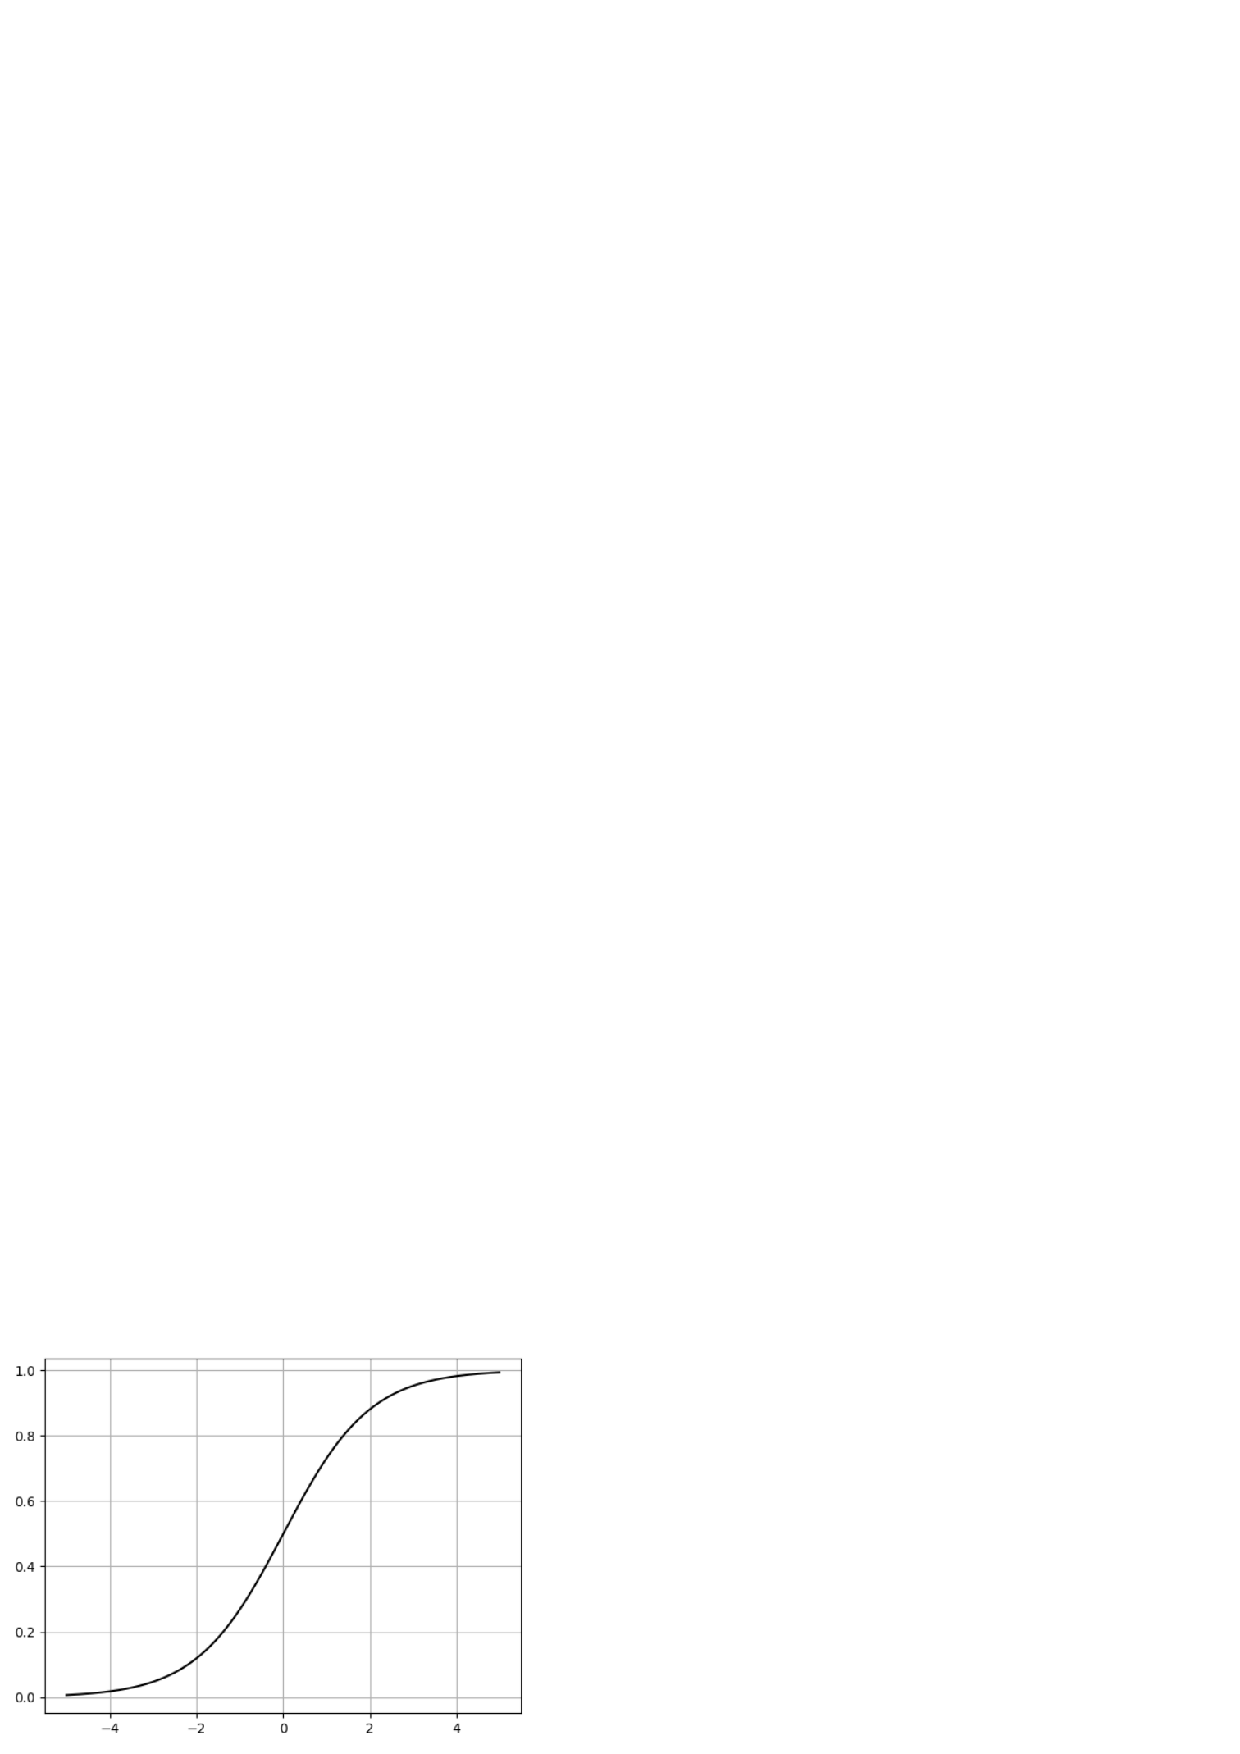
\includegraphics[width=0.3\textwidth]{./fig/Sigmoid}
    \label{subfig:sigmoid}
   }
   \captionsetup{width=1\textwidth}
   \caption{{\subref{subfig:relu}}, {\subref{subfig:tanh}} e {\subref{subfig:sigmoid}} representam o comportamento das funções de ativação ReLU, TanH e Sigmóide, respectivamente \cite{Luckeciano}.}
  \label{fig:activationfunctions}
\end{figure}

% \subsection{Topologia}
Uma rede neural combina diversos neurônios em diversas camadas, formando um grafo direcionado (tipicamente acíclico) por onde os dados fluem. Os neurônios de uma camada processam os dados de entrada e passam os resultados como entrada dos neurônios da próxima camada, até encontrar a camada de saída \cite{MichaelNielsen}. Uma rede neural que possui muitas camadas é denominada uma Rede Neural Profunda. A Figura \ref{fig:neuralnetworks} ilustra o fluxo de processamento de redes neurais.

\begin{figure}[ht]
 \centering
  \subfigure[Rede neural.]
   {
    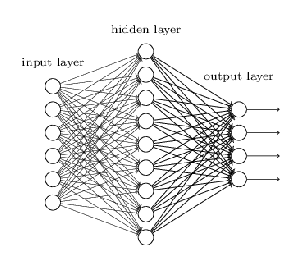
\includegraphics[width=0.35\textwidth]{./fig/NeuralNetwork}
    \label{subfig:nn}
   } \qquad
  \subfigure[Rede neural profunda.]
   {
    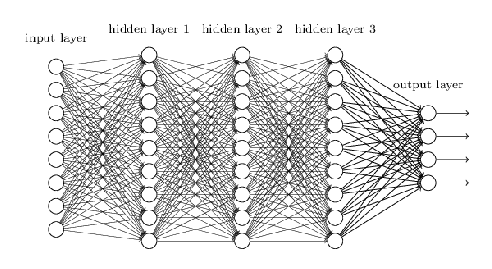
\includegraphics[width=0.55\textwidth]{./fig/DNN}
    \label{subfig:deepnn}
   }
   \captionsetup{width=1\textwidth}
   \caption{{\subref{subfig:nn}} e {\subref{subfig:deepnn}} representam uma rede neural convencional e uma rede neural profunda, respectivamente \cite{MichaelNielsen}.}
  \label{fig:neuralnetworks}
\end{figure}

Existem diversas topologias para redes neurais que não seguem necessariamente a configuração apresentada. Redes Neurais Convolucionais, por exemplo, utilizam filtros convolucionais para extrair características em conjuntos de entradas onde a posição dos elementos é importante (e.g. imagens) \cite{LeCun1989} e Redes Neurais Recorrentes definem grafos cíclicos para modelagem de dados em domínios temporais \cite{Rumelhart1986}. As camadas de uma rede neural podem ter todos os seus neurônios conectados a todos os neurônios da camada anterior - as camadas densas - ou podem ter conexões compartilhadas, como é o caso dos filtros convolucionais \cite{LeCun1989}.

\begin{figure}[ht]
 \centering
  \subfigure[Topologia de uma Neural Convolucional.]
   {
    \includegraphics[width=0.55\textwidth]{./fig/CNN}
    \label{subfig:convnn}
   } \qquad
  \subfigure[Topologia de uma Rede Neural Recorrente.]
   {
    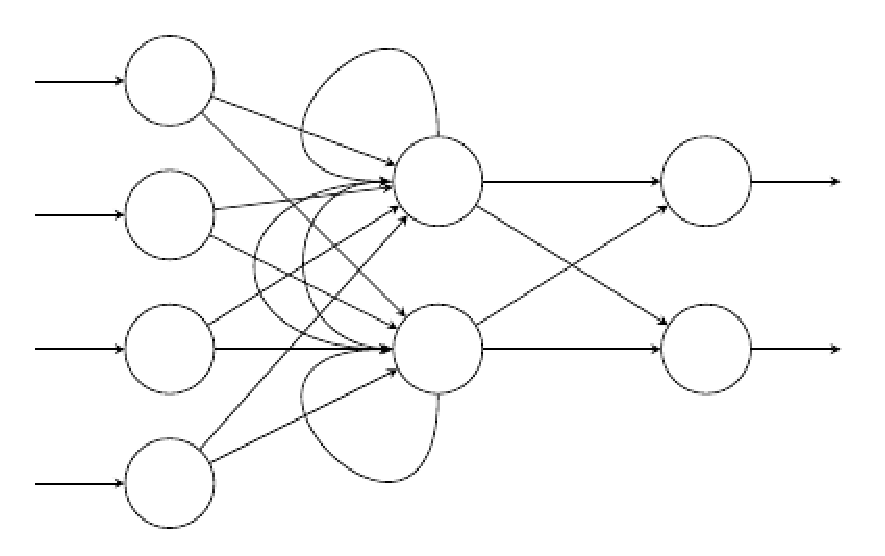
\includegraphics[width=0.35\textwidth]{./fig/RNN}
    \label{subfig:rnn}
   }
   \captionsetup{width=1\textwidth}
   \caption{{\subref{subfig:convnn}} e {\subref{subfig:rnn}} representam diferentes topologias que redes neurais podem assumir.}
  \label{fig:topologies}
\end{figure}

% \subsection{Otimização}

A otimização, ou treinamento, de redes neurais é uma tarefa natural do aprendizado supervisionado, que será introduzido em seguida. Os algoritmos mais utilizados para isso são baseados na propagação do gradiente de uma função de custo através da rede a fim de atualizar seus parâmetros e minimizar esta função, um processo conhecido como \textit{backpropagation} \cite{Goodfellow2016}.

%% - - - - - - - - - - - - - - - - - - - - - - - - - - - - - - - - - - -

\section{Aprendizado de Máquina}
\label{sec:aprendizadomaquina}

Aprendizado de máquina é um subcampo da Inteligência Artificial que estuda a capacidade de algoritmos aprenderem a executar tarefas baseadas em dados sem que sejam explicitamente programados para tal \cite{Simon2013TooBT}. Na prática, seu objetivo é modelar teórica e matematicamente o processo de melhoria interativa das aplicações, baseando-se em padrões intrínsecos dos dados disponíveis. Existem três principais técnicas para alcançar este objetivo: aprendizado supervisionado, aprendizado não supervisionado e aprendizado por reforço. 

No aprendizado supervisionado pares de exemplos no formato $(X, Y)$, onde $X$ são entradas e $Y$ são saídas, são dados ao algoritmo para que este consiga aproximar uma função $f$ que mapeie uma entrada $x \in X$ à saída correspondente $y \in Y$ \cite{Russel}. Algoritmos de aprendizado supervisionado podem ainda ser classificados entre algoritmos de classificação e algoritmos de regressão, onde o primeiro mapeia uma entrada $x$ a uma das classes em $Y$ e o segundo mapeia uma entrada $x$ em um valor contínuo no domínio de $Y$.

No aprendizado não supervisionado, por sua vez, o aprendizado é feito sobre dados não anotados, ou seja, sem o conjunto $Y$. O objetivo dessa classe de algoritmos é extrair padrões e regras, agrupar ou resumir os dados \cite{Russel}.

Já no aprendizado por reforço o aprendizado ocorre através da interação com um ambiente. Uma solução para um problema de aprendizado por reforço - o agente - deve interagir com o ambiente executando ações que geram sinais de recompensa. Dessa forma, o agente, em busca de maximizar o valor total da soma de suas recompensas futuras, deve aprender comportamentos (políticas) que ao mesmo tempo resolvem o problema inicialmente proposto \cite{Russel}. A Figura \ref{fig:reinforcementfig} representa o processo descrito. Esta abordagem é descrita em mais detalhes na Seção \ref{sec:reinforcementlearning}.
\begin{figure}[ht]
 \centering
  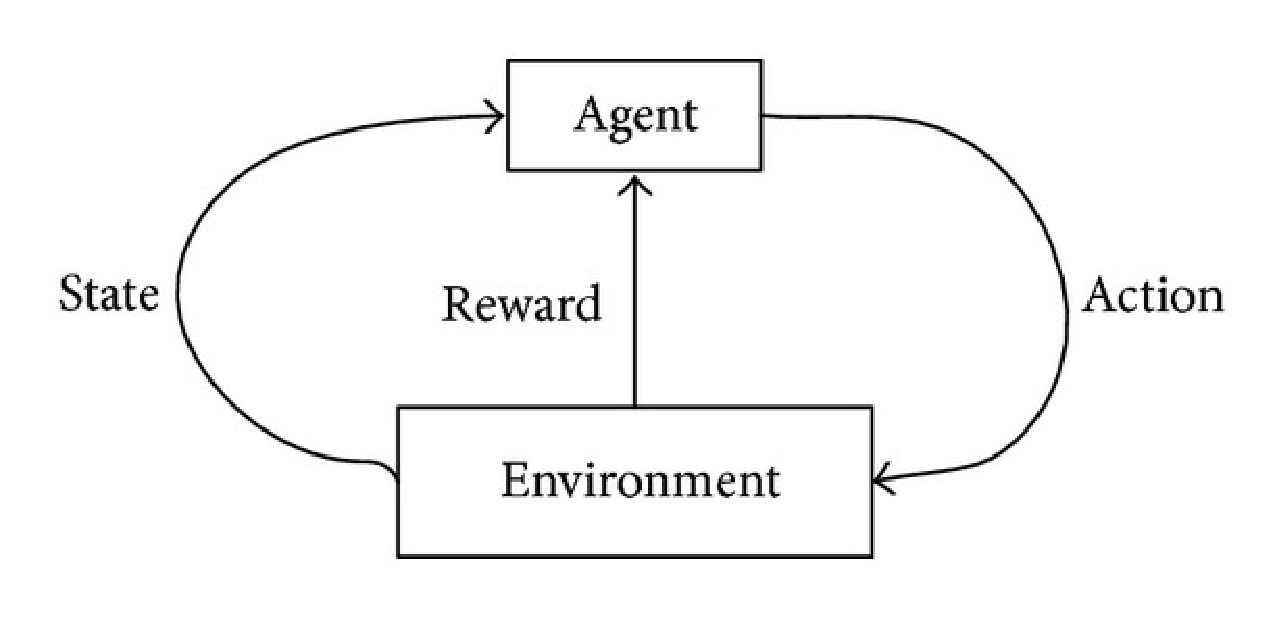
\includegraphics[width=0.70\textwidth]{./fig/Framework-of-reinforcement-learning-Agent-selects-an-action-the-environment-responds-to}
  \captionsetup{width=1\textwidth}
  \caption[Diagrama do processo de aprendizado por reforço \cite{ZhouXiaoke}.]{Diagrama do processo de aprendizado por reforço \cite{ZhouXiaoke}. Um agente (\textit{Agent}), em um dado estado (\textit{State}), seleciona ações (\textit{Action}) que são aplicadas no ambiente (\textit{Environment}) que, por sua vez, retorna um novo estado e um sinal de recompensa (\textit{Reward}) para o agente.}
 \label{fig:reinforcementfig}
\end{figure}

%% - - - - - - - - - - - - - - - - - - - - - - - - - - - - - - - - - - -

\section{Aprendizado por Reforço}
\label{sec:reinforcementlearning}

No aprendizado por reforço, um agente aprende através de sua interação com o ambiente em sequências de iterações, chamadas de episódios. Essa interação é tipicamente modelada como um Processo de Decisão de Markov (MDP), definido por um conjunto de estados $S$, um espaço de ações $A$, uma função de recompensa $r: S \times A \rightarrow [-\infty, \infty)$, um fator de desconto $\gamma \in [0, 1)$ e uma função de transição $P: S \times A \rightarrow \Delta(S)$. Nessa configuração, $\Delta(S)$ é o espaço de distribuições de probabilidade $P(s'|s, a)$ de transição para um estado $s'$ a partir de um estado $s$ e executando a ação $a$. O fator de desconto $\gamma$ é utilizado para balancear quanto um agente deve priorizar recompensas imediatas ou recompensas futuras. A Figura \ref{fig:mdp} ilustra o sistema descrito.

\begin{figure}[ht]
 \centering
  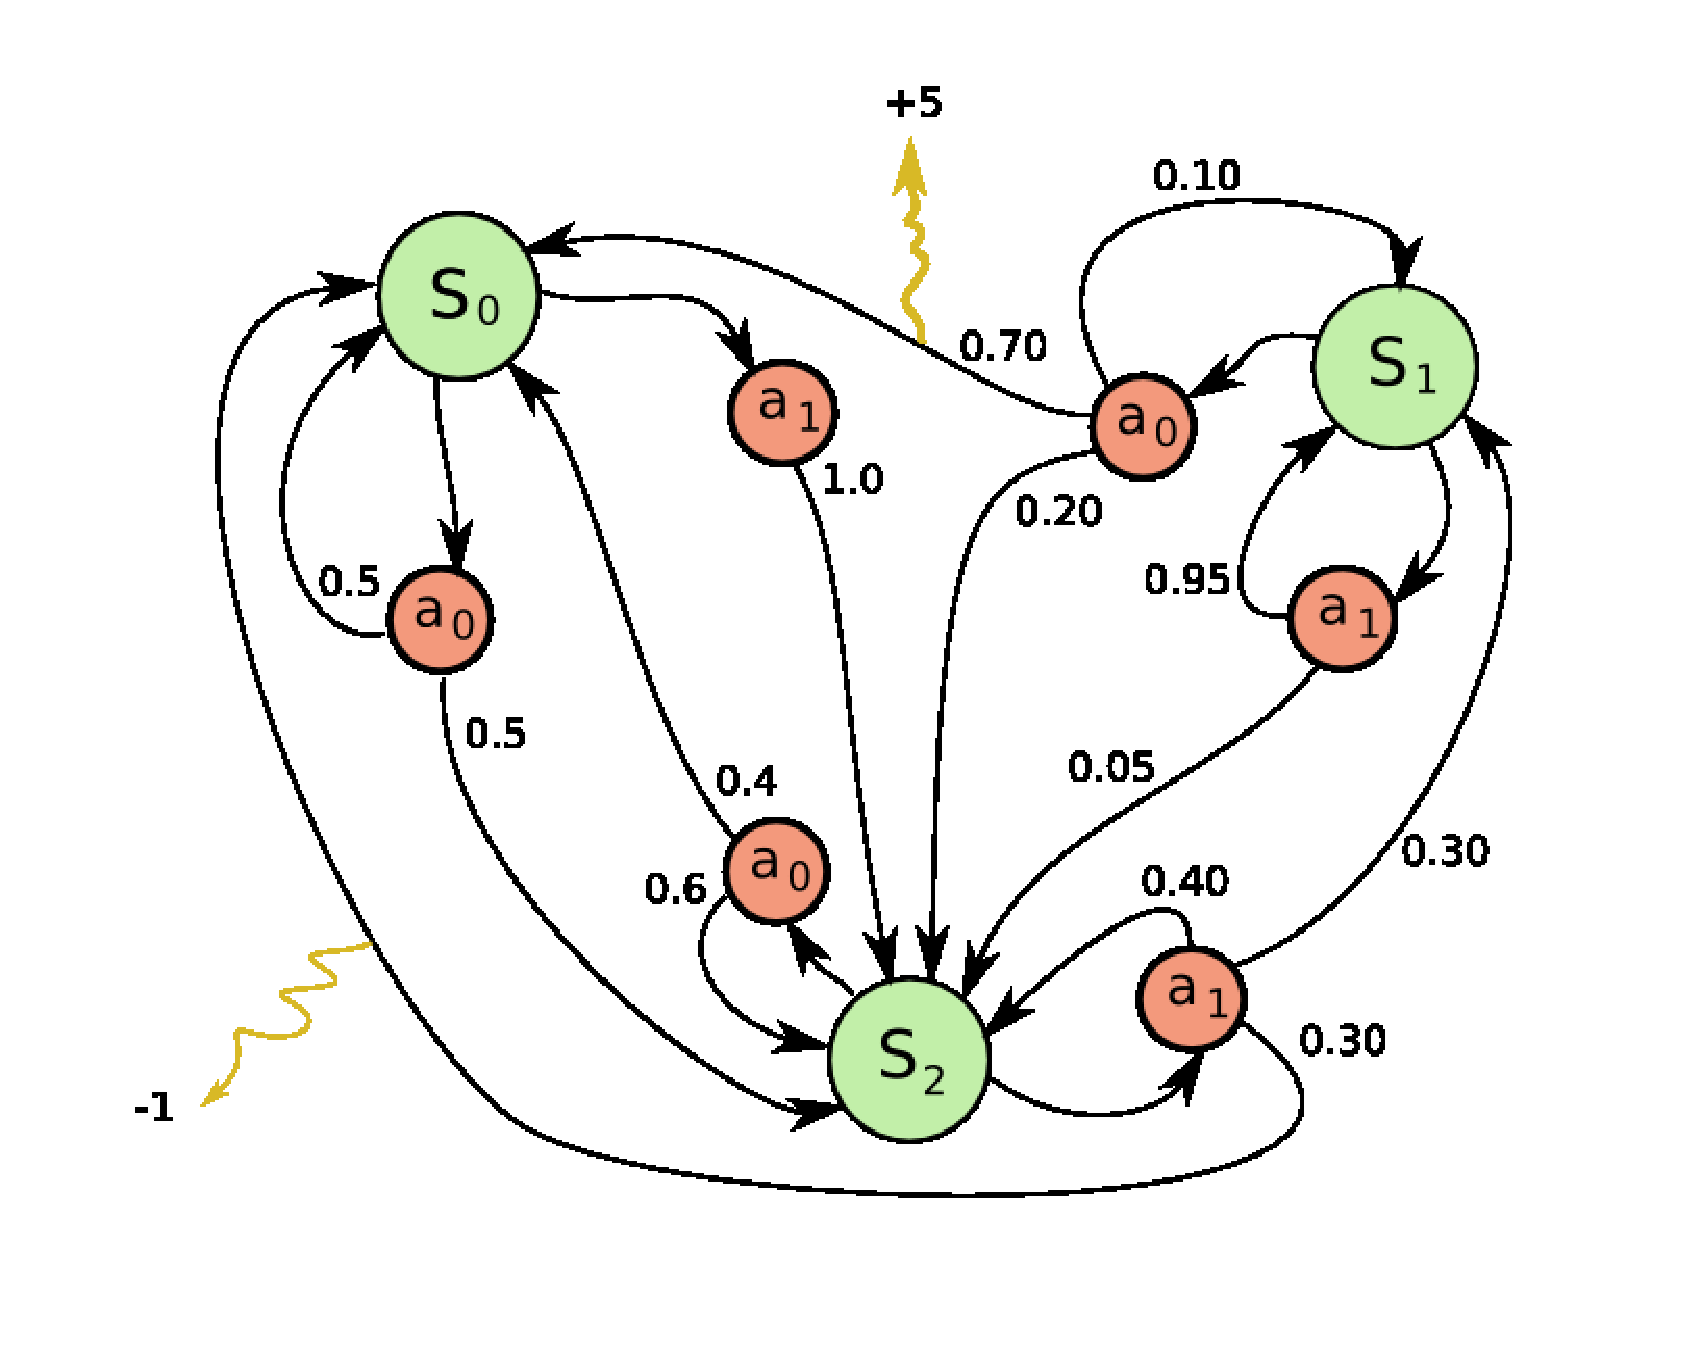
\includegraphics[width=0.6\textwidth]{./fig/mdp}
  \captionsetup{width=1\textwidth}
  \caption[Um Processo de Decisão de Markov \cite{mohammad}.]{Um Processo de Decisão de Markov \cite{mohammad}. Os estados $s_i \in S$ e as ações $a_i \in A$ são representadas pelos vértices verdes e vermelhos, respectivamente. Os valores das arestas são as probabilidades de transição $P$ e os valores indicados pelas setas amarelas são as recompensas obtidas em cada transição.}
 \label{fig:mdp}
\end{figure}

Sequências de transições em um MDP formam uma cadeia de Markov \cite{drlhandson}. O valor total de recompensas, ou retorno, que um agente pode receber em uma cadeia a partir de um tempo $t$ é definido pela Equação \ref{eqn:rewards}.

\begin{equation}
\label{eqn:rewards}
R_t = r_{t+1} + \gamma r_{t+2} + ... = \sum^\infty_{k=0}{\gamma^k r_{t+k+1}}
\end{equation}

Na prática, diferentes cadeias de transições podem resultar no mesmo valor de $R_t$. Como o objetivo de um agente de aprendizado por reforço é maximizar o retorno para uma cadeia qualquer, definimos, para esse fim, a função de valor $V$ para um estado $s$, como mostra a Equação \ref{eqn:value}. O valor de um estado, portanto, pode ser definido como o valor esperado da recompensa que pode ser acumulada a partir do estado atual, independentemente da sequência exata de transições que ocorreram.

\begin{equation}
\label{eqn:value}
V(s) = \mathop{{}\mathbb{E}} [R | S_t=s]
\end{equation}

O agente seleciona suas ações baseando-se em sua política, que pode ser determinística, como na Equação \ref{eqn:pidet}, ou estocástica, como na Equação \ref{eqn:piest}. Tipicamente, políticas determinísticas são utilizadas em ambientes determinísticos, como o jogo de xadrez, enquanto que políticas estocásticas são amplamente utilizadas em ambientes estocásticos, como em um jogo de poker, modelados como Processos de Decisão de Markov Parcialmente Observáveis (PDMPO) \cite{drlhandson}. Em MDPs, a observação do estado atual é suficiente para que um agente obtenha uma política ótima, ou seja, é suficiente para que seja possível alcançar o objetivo de maximizar sua recompensa acumulada. PDMPOs, por outro lado, possuem variáveis escondidas que tornam essa tarefa significativamente difícil e, portanto, são abordados com estratégias mais sofisticadas.

\begin{equation}
\label{eqn:pidet}
\pi(s) = a
\end{equation}

\begin{equation}
\label{eqn:piest}
\pi(a|s) = P(A_t=a | S_t=s)
\end{equation}

Um agente pode otimizar seu comportamento melhorando sua estimativa do valor de um par estado-ação (métodos baseados em valor) ou modificando sua política (métodos baseados em política). Além disso, um agente pode armazenar e otimizar um modelo do ambiente internamente (baseado em modelo) para consultá-lo na tomada de decisões ou trabalhar sem conhecer o funcionamento interno do ambiente (livre de modelo). Outro tipo de classificação especifica se o agente utiliza informações da própria política exploratória para otimização em direção à política ótima (\textit{on-policy}) ou não (\textit{off-policy}) \cite{suttonbarto}.

Agentes modernos de aprendizado por reforço tipicamente utilizam redes neurais como forma de parametrizar seus componentes. Isso permite que o agente trabalhe com espaços de observação e ação contínuos e de alta dimensionalidade. Esses agentes são comumente denominados agentes de aprendizado por reforço profundo. Uma política parametrizada por parâmetros $\theta$ é denotada por $\pi_\theta$.

Enxergando a otimização de agentes como um problema de maximização de recompensa acumulada, técnicas de exploração dão ao agente a possibilidade de sair de máximos locais ao explorar novos estados do ambiente. Uma das políticas exploratórias mais utilizadas é o $\epsilon$-\textit{greedy} \cite{egreedy}. Nessa técnica, o agente seleciona a ação de maior valor estimado com probabilidade $1-\epsilon$ ou uma ação aleatória com probabilidade $\epsilon$, como é feito em \cite{deepq}. Ao decorrer do processo de treinamento, o parâmetro $\epsilon$ é reduzido até que somente a política do agente seja utilizada na seleção de ações. 

Em métodos baseados em política, a exploração pode ser feita através da seleção da ação por amostragem em uma distribuição de probabilidades gerada pela política. Nesse método, a ação executada em um estado pode variar, mas de forma controlada. Outra forma de encorajar a exploração em métodos baseados em política é a adição de um termo de regularização baseado na entropia ($H(\pi(s_t; \theta))$) da distribuição gerada pelo agente na função de custo do problema de otimização da política \cite{a3c, williamspeng}. Isso faz com que o agente prefira distribuições mais uniformes a distribuições que encorajam demais as mesmas ações, evitando a convergência (ou seja, a estabilização em resultados relativamente satisfatórios) para políticas sub-ótimas e mantendo um nível controlado de exploração \cite{a3c, williamspeng}.

\section{Estimativa de Vantagem Generalizada}
\label{sec:gae}

Métodos baseados em política possuem a vantagem de aprender políticas estocásticas, ao contrário de métodos baseados em valor. Além disso, esses métodos conseguem trabalhar em espaços de ação de alta dimensionalidade, ou contínuos, por poderem ser representados por qualquer aproximador parametrizado que mapeie estados a ações \cite{suttonbarto}. Métodos baseados em política selecionam suas ações sem consultar diretamente uma função de valor, mas comumente as utilizam internamente no processo de otimização. Outra vantagem de utilizar métodos baseados em política é sua garantia de convergência pelo método de Gradiente de Política \cite{policygradients}.

Métodos modernos de Gradiente de Política utilizam como objetivo, assim como os métodos tradicionais de aprendizado por reforço, a maximização da recompensa obtida pelo agente. Para isso, no entanto, é utilizada a Estimativa de Vantagem Generalizada (GAE) \cite{gae}, definida pela Equação \ref{eqn:gae}. Nesse contexto, definimos a vantagem $A$ para um tempo $t$ como a diferença entre a estimativa de valor para o estado atual e o real valor obtido empiricamente. Essa função nos diz se a recompensa obtida foi melhor ($A > 0$) ou pior ($A < 0$) que a recompensa esperada pelo agente. Se for melhor, devemos reforçar as ações executadas no episódio. Se for pior, devemos tornar essas ações menos prováveis.

\begin{equation}
\label{eqn:gae}
A_t^{GAE(\gamma, \lambda)} = (1 - \lambda)(A_t^{(1)} + \lambda A_t^{(2)} + \lambda^2A_t^{(3)} + ...)
\end{equation}

Aqui, $A_t^{GAE(\gamma, \lambda)}$ é um estimador para a função de vantagem generalizada, aplicado no tempo $t$ e configurado pelos hiperparâmetros $\gamma$ e $\lambda$. Os estimadores de vantagem com visão de $n$ passos a partir do tempo $t$ ($A^{(n)}$) são definidos pela Equação \ref{eqn:nstepadv}. O hiperparâmetro $\lambda$ varia de 0 a 1 e controla quanto das estimativas de vantagem para passos futuros devem ser considerados, balanceando o viés e a variação das estimativas \cite{gae}.

\begin{equation}
\label{eqn:nstepadv}
A_t^{(n)}(s, a) = r_t + \gamma V(s_{t+1}) + ... + \gamma^n V(s_{t+n}) - V(s_t)
\end{equation}

O uso de estimadores de vantagem para a otimização nos métodos de Gradiente de Política torna o treinamento mais estável em relação ao uso dos retornos (Equação \ref{eqn:rewards}) para valores de $\lambda$ entre 0 e 1 \cite{gae}.

\section{Proximal Policy Optimization}
\label{sec:ppo}

Um recorrente problema no treinamento de redes neurais é a escolha da taxa de aprendizado. Este parâmetro controla quanto o gradiente influencia na modificação dos parâmetros da rede e é bastante sensível: se for muito grande, a rede pode ser modificada drasticamente e perdemos qualquer conhecimento adquirido até o momento; se for muito pequeno, o treinamento é muito lento.
Esse efeito é ainda maior no aprendizado por reforço, em especial em métodos baseados em política. Leves mudanças nos parâmetros podem levar a grandes mudanças no comportamento do agente, o que torna o treinamento um processo instável.

O algoritmo \textit{Proximal Policy Optimization} (PPO) \cite{ppo} foi introduzido com o propósito de mitigar justamente esse problema, limitando a mudança sofrida pela política entre as atualizações de seus parâmetros. A proporção da atualização da nova política em relação a política anterior é dada pela Equação \ref{eqn:pporatio}.

\begin{equation}
\label{eqn:pporatio}
d_t(\theta) = \frac{\pi_\theta(a_t|s_t)}{\pi_{\theta_{old}}(a_t|s_t)}
\end{equation}

Nesse contexto, se $d_t(\theta)$ > 1, então a ação $a_t$ é mais provável na política atual do que na política antiga. Por outro lado, se $0 < d_t(\theta) < 1$, a ação $a_t$ é menos provável na política atual do que na política antiga. Com base nisso, definimos a função de atualização limitada do PPO na Equação \ref{eqn:ppoloss}, onde \textit{clip} é uma função de corte que restringe $d_t$ ao intervalo $(1-\epsilon, 1+\epsilon)$.

\begin{equation}
\label{eqn:ppoloss}
L^{CLIP}(\theta) = \mathop{{}\mathbb{E}}{}_t [min(d_t(\theta)A_{\pi_\theta}, clip(d_t(\theta), 1-\epsilon, 1+\epsilon) A_{\pi_\theta})]
\end{equation}

Essa função é calculada por N passos de otimização sobre um lote de iterações coletado durante um episódio. Como o objetivo do PPO é garantir pequenas atualizações nos parâmetros $\theta$ a cada episódio, a função de atualização busca o mínimo entre uma atualização para o passo atual com e sem o limite de proporção $\epsilon$. Isso desencoraja a política de desviar muito do que era, uma vez que os gradientes zeram ao ultrapassar a região de corte, como mostra a Figura \ref{fig:ppoclip}. Em outras palavras, se a ação foi boa ($A > 0$) e se tornou mais provável após o último passo de otimização do gradiente, é permitido aumentar sua probabilidade ainda mais até que $d_t$ atinja o limite de corte $1+\epsilon$, ou diminuí-la para reparar erros de passos anteriores. Da mesma forma, se a ação foi ruim ($A < 0$) e se tornou menos provável, é permitido diminuir sua probabilidade até que $d_t$ atinja o limite de corte $1-\epsilon$, ou aumentá-la para reparar erros de passos anteriores.

\begin{figure}[ht]
 \centering
  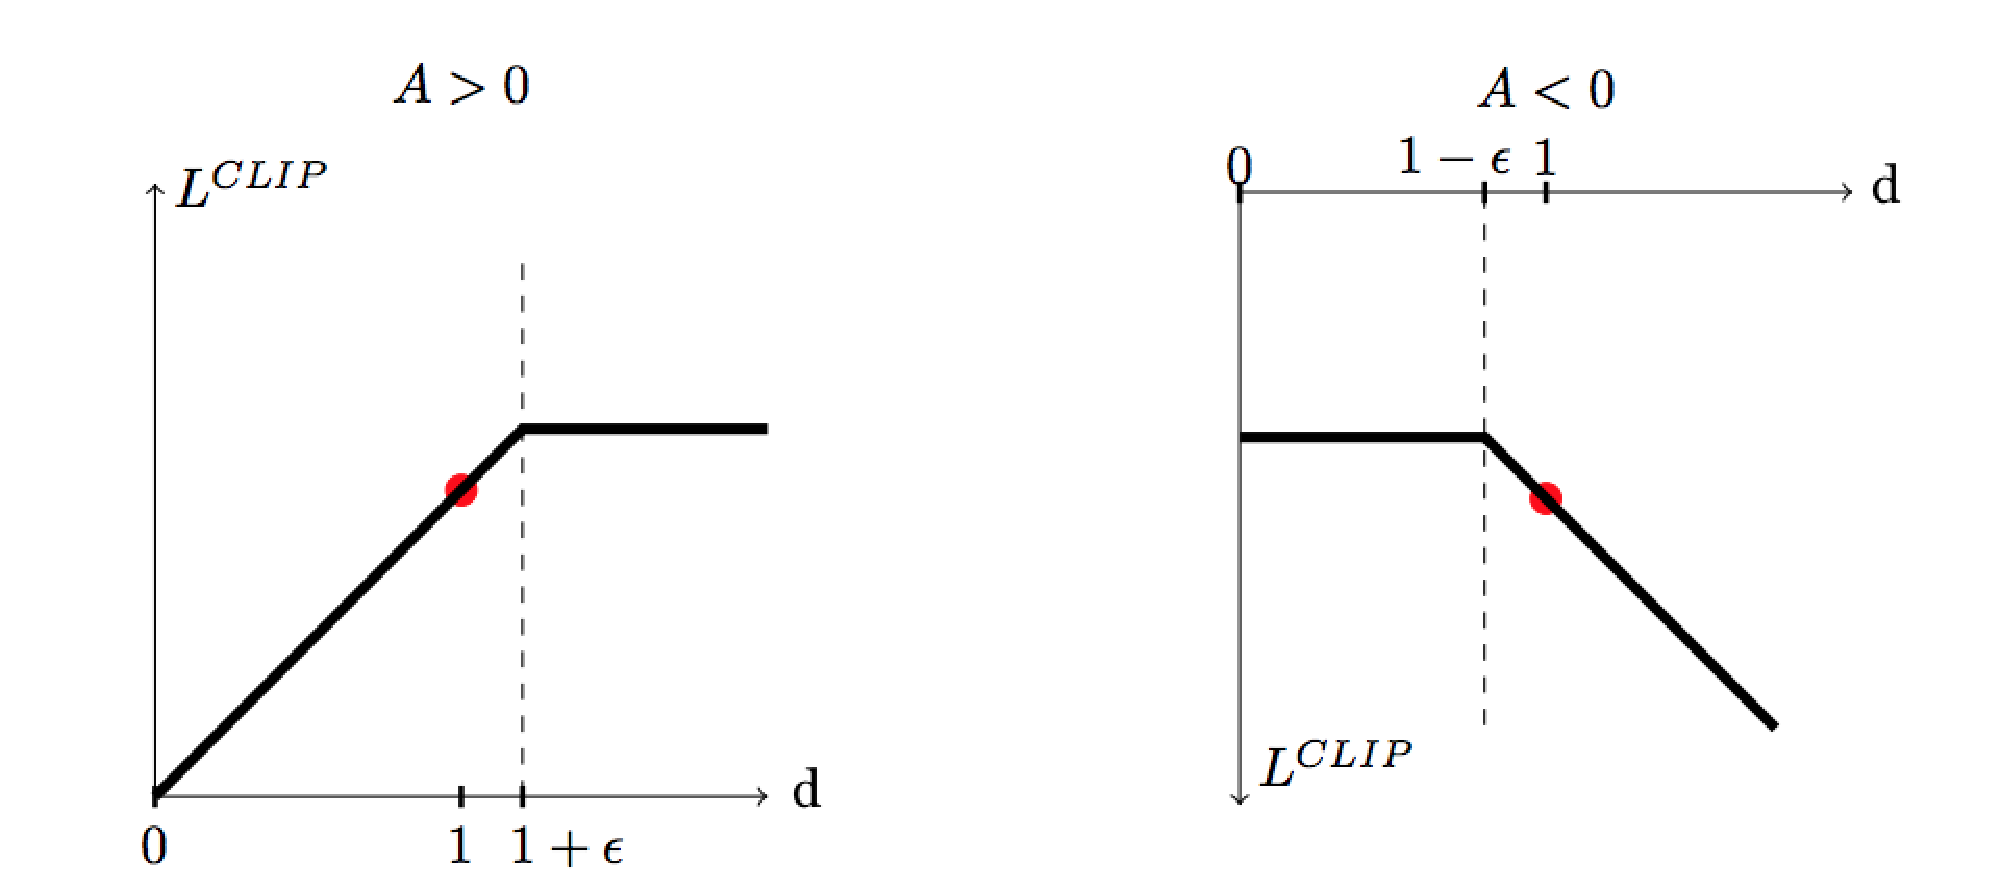
\includegraphics[width=0.8\textwidth]{./fig/ppo_clip}
  \captionsetup{width=1\textwidth}
  \caption{Comportamento da função $L^{CLIP}$ para valores de vantagem positivos (esquerda) e negativos (direita) \cite{ppo}, para atualizações em um único episódio.}
 \label{fig:ppoclip}
\end{figure}

Neste trabalho, a função de atualização do PPO é combinada com o termo de regularização baseado na entropia, definido na Seção \ref{sec:gae}. Além disso, um modelo parametrizado que estima a função de valor $V$ também é otimizado, caracterizando assim uma arquitetura Ator-Crítico \cite{suttonbarto}. A função de atualização toma então a forma da Equação \ref{eqn:totalloss}, onde $c$ é uma constante que regula a escala do termo de entropia e $L^{VF}$ é a função de custo do modelo da função de valor.

\begin{equation}
\label{eqn:totalloss}
L^{CLIP + VF + H}(\theta) = \mathop{{}\mathbb{E}}{}_t [L^{CLIP} - L^{VF} + cH(\pi(s_t; \theta))]
\end{equation}

Por fim, o algoritmo PPO com função de atualização limitada é apresentado no Algoritmo \ref{alg:ppoclip} \cite{achiam}, onde N é o tamanho do lote de treinamento do algoritmo de otimização.

\medskip
\begin{center}
\begin{minipage}{0.92\textwidth}
\begin{algorithm2e}[H]
 \DontPrintSemicolon
 \Entrada{parâmetros da política inicial $\theta_0$, limiar de corte $\epsilon$}
 \Para{$k= 0, 1, 2, ...$}
   {Colete um conjunto de trajetórias $D_k$ com política $\pi_k = \pi(\theta_{k})$ \\
    Estime a função de vantagem $A_{t}^{GAE(\gamma, \lambda)}$ \\
    Calcule a atualização da política \\
    \hspace{2cm}$\theta_{k+1} = arg \max_{\theta} L^{CLIP + VF + H}(\theta_k)$ \\
    executando N passos do gradiente ascendente, onde \\
    \hspace{2cm}$L^{CLIP + VF + H}(\theta_k) = \mathop{{}\mathbb{E}}{}_t [L^{CLIP} - L^{VF} + cH(\pi(s_t; \theta))]$ 
   }
\caption{PPO com função de atualização limitada \label{alg:ppoclip} }
\end{algorithm2e}
\end{minipage}
\end{center}



\section{Motivação Intrínseca}
\label{sec:curiosidade}

Um dos maiores desafios do aprendizado de reforço é aplicação de suas técnicas em ambientes reais. Dois principais problemas podem ser destacados: generalização e modelagem de recompensa. O primeiro diz respeito a capacidade de um agente treinado em uma configuração específica, ou um simulador, ser capaz de atuar de forma satisfatória em diferentes configurações, como em um manipulador robótico real. O segundo diz respeito à dificuldade de se modelar funções de recompensa que guiem um agente a agir de forma a completar uma determinada tarefa.

A sensibilidade dos algoritmos de aprendizado por reforço ao segundo problema faz com que, na maioria das vezes, o agente aprenda a explorar falhas do simulador ou falhas da modelagem da recompensa e simplesmente ignorar a tarefa que lhe foi dado. Além disso, a modelagem da função de recompensa para tarefas minimamente complexas é uma tarefa difícil \cite{dexterity, ng, deepLoco}. A alternativa natural é o uso de recompensas esparsas, recompensando o agente apenas no momento em que ele completou a tarefa desejada, por exemplo. Porém, em ambientes onde a recompensa é esparsa ou inexistente, aprender boas políticas por tentativa e erro é uma tarefa extremamente difícil. Nessas situações, não existe um direcionamento claro de como o agente deve modificar sua política a fim de maximizar sua recompensa. Além disso, técnicas de exploração clássicas comumente utilizam distribuições de probabilidade sobre as ações que não levam em consideração guiar o agente a estados inexplorados, o que pode não ser suficiente para a descoberta de políticas que são capazes de alcançar o objetivo determinado \cite{pathak}.

Como saída para este problema é possível encorajar o agente a explorar melhor o ambiente e aprender novas habilidades recompensando-o de forma intrínseca, ou seja, independente da recompensa fornecida pelo ambiente (extrínseca). Uma forma de modelar a motivação intrínseca é através da geração um sinal de recompensa proporcional ao nível de surpresa do agente em relação aos estados que ele observa \cite{curiosityoriginal, pathak}. Para isso, um modelo de futuro é responsável por prever o próximo estado $s_{t+1}$ dados o estado atual $s_t$ e a ação $a$ executada, como mostra a Equação \ref{eqn:forward}.

\begin{equation}
\label{eqn:forward}
\hat{s}_{t+1} = f(s_t, a_t; \theta_F)
\end{equation}

Dado o real estado futuro $s_{t+1}$ é calculado o erro de predição, ou seja, a função de custo do modelo, como mostra a Equação \ref{eqn:curiosityloss}.

\begin{equation}
\label{eqn:curiosityloss}
L_F(s_{t+1}, \hat{s}_{t+1}) = \frac{1}{2}\|\hat{s}_{t+1} - s_{t+1}\|_2^2
\end{equation}

O erro de predição é então multiplicado por uma constante $\eta$ que ajusta sua escala. Por fim, o valor é adicionado à recompensa do ambiente ($r^e$) como recompensa intrínseca, como mostra a Equação \ref{eqn:curiosityreward}.

\begin{equation}
\label{eqn:curiosityreward}
r_t = r^e_t(s_t, a, s_{t+1}) + \eta L_F
\end{equation}
\chapter{Materiais e Métodos}
\label{cap:metodologia}

Utilizando como base os conceitos previamente abordados, este Capítulo descreve os ambientes de \textit{benchmark} utilizados para experimentação, o funcionamento do algoritmo utilizado e os testes executados. Primeiramente, são apresentados os objetivos do agente nos ambientes escolhidos e como é configurada a observação e a recompensa, assim como o espaço de ações e a duração do episódio. Em seguida, o algoritmo PPO é retomado e modificado para incluir o módulo de motivação intrínseca. O funcionamento geral dos passos do algoritmo são descritos em mais detalhes e a arquitetura das redes neurais utilizada é apresentada. Por fim, os testes são descritos e as hipóteses deste trabalho são estabelecidas, assim como o comportamento esperado de cada métrica a ser analisada.

% - - - - - - - - - - - - - - - - - - - - - - - - - - - - - - - - - - -

\section{OpenAI Gym}
\label{sec:gym}

\begin{figure}[hb]
 \centering
  \subfigure[CartPole.]
   {
    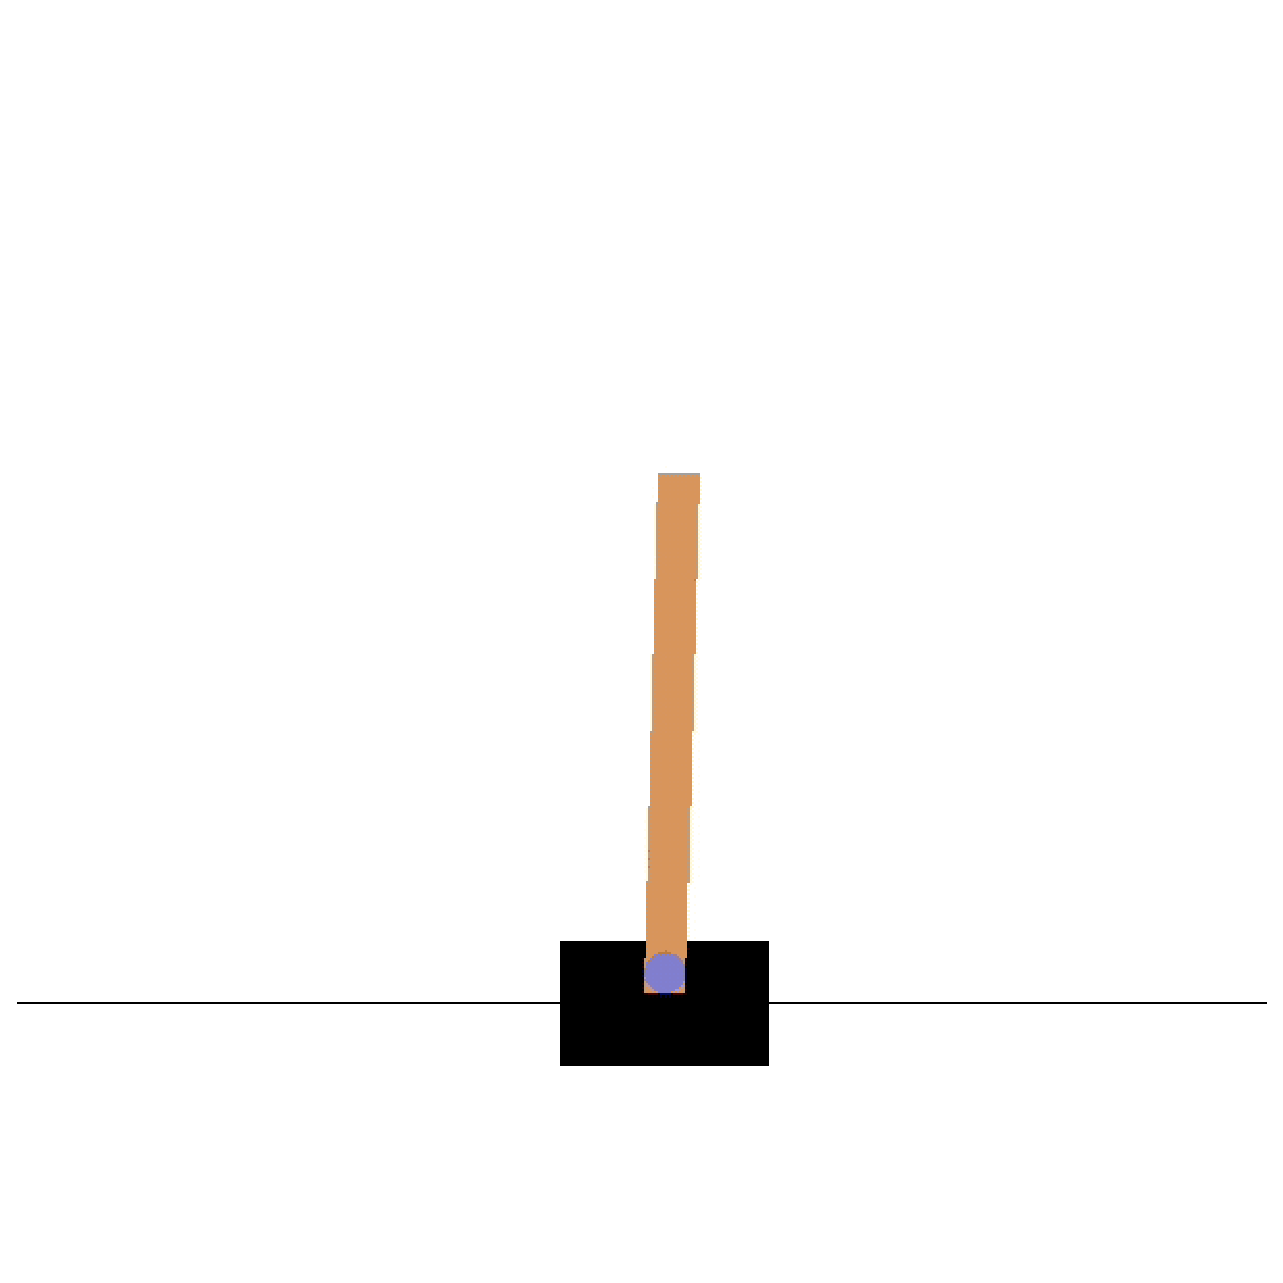
\includegraphics[width=0.35\textwidth]{./fig/cartpole-0}
    \label{subfig:cartpole}
   } \qquad
  \subfigure[HandManipulateBlock.]
   {
    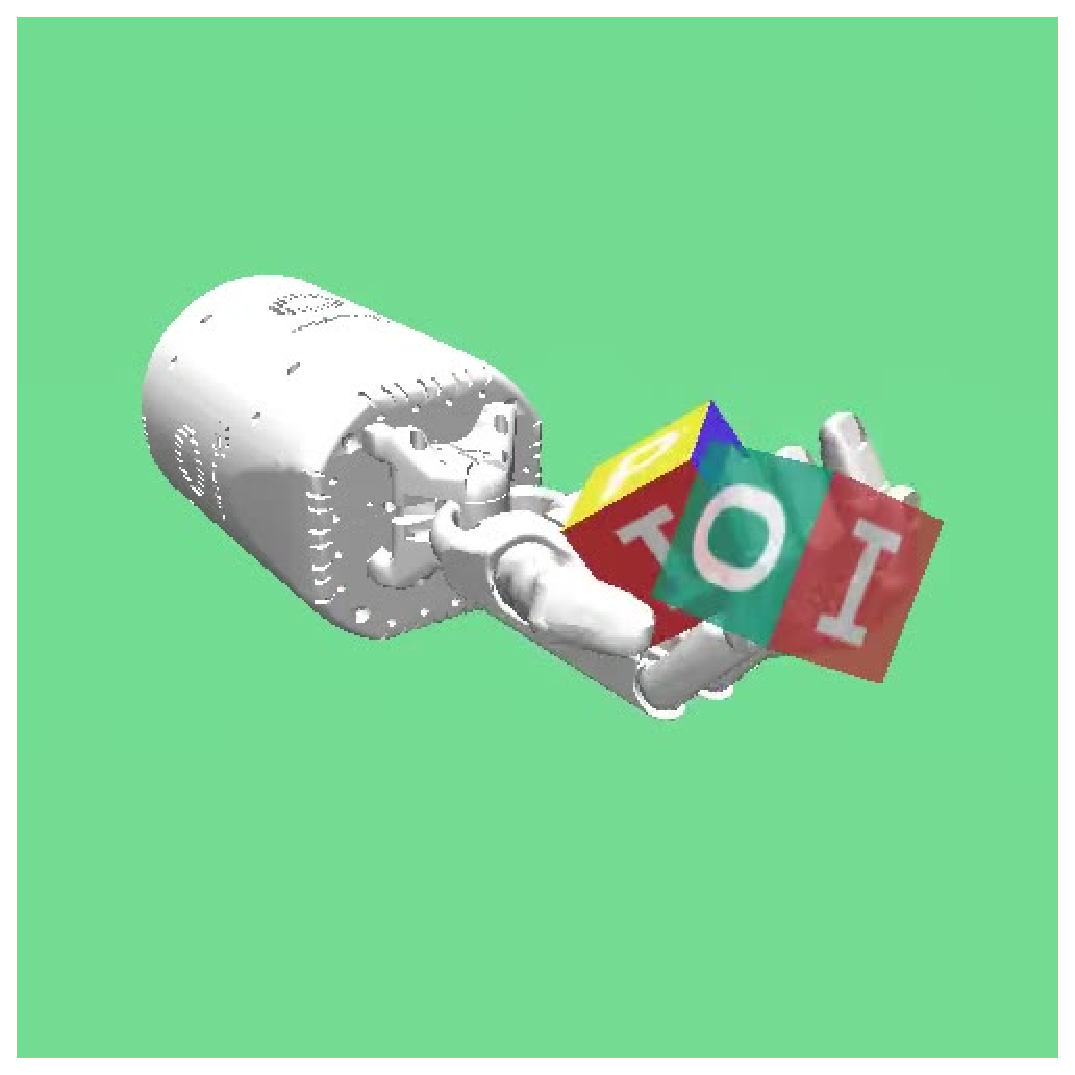
\includegraphics[width=0.35\textwidth]{./fig/handmanipulate}
    \label{subfig:handmanipulate}
   }
   \captionsetup{width=1\textwidth}
   \caption[Ambientes do Gym.]{Ambientes do Gym. Em {\subref{subfig:cartpole}}, o agente deve equilibrar a estaca selecionando ações entre [esquerda, direita]. Em {\subref{subfig:handmanipulate}}, o agente deve posicionar o bloco opaco como mostra o bloco translúcido de exemplo, selecionando valores de torque para cada junta da mão.}
  \label{fig:gymenvs}
\end{figure}

O OpenAI Gym \cite{gym} é uma ferramenta de \textit{benchmark} para algoritmos de aprendizado por reforço que tem como objetivo ser agnóstico em relação à estrutura dos agentes e manter uma interface amigável e comum a seus diversos ambientes. O Gym inclui ambientes que variam desde problemas simples, como o famoso \textit{CartPole} (Figura \ref{subfig:cartpole}), até simulações de mãos robóticas, como o \textit{HandManipulateBlock} (Figura \ref{subfig:handmanipulate}).

Para os testes deste trabalho, foram escolhidos ambientes de manipulação robótica \textit{FetchReach}, \textit{FetchPush}, \textit{FetchPickAndPlace}, ilustrados pela Figura \ref{fig:fetchenvs}. A escolha desses ambientes possibilita a avaliação da aplicabilidade de técnicas similares a apresentada neste trabalho em manipuladores reais.

\begin{figure}[ht]
 \centering
  \subfigure[FetchReach.]
   {
    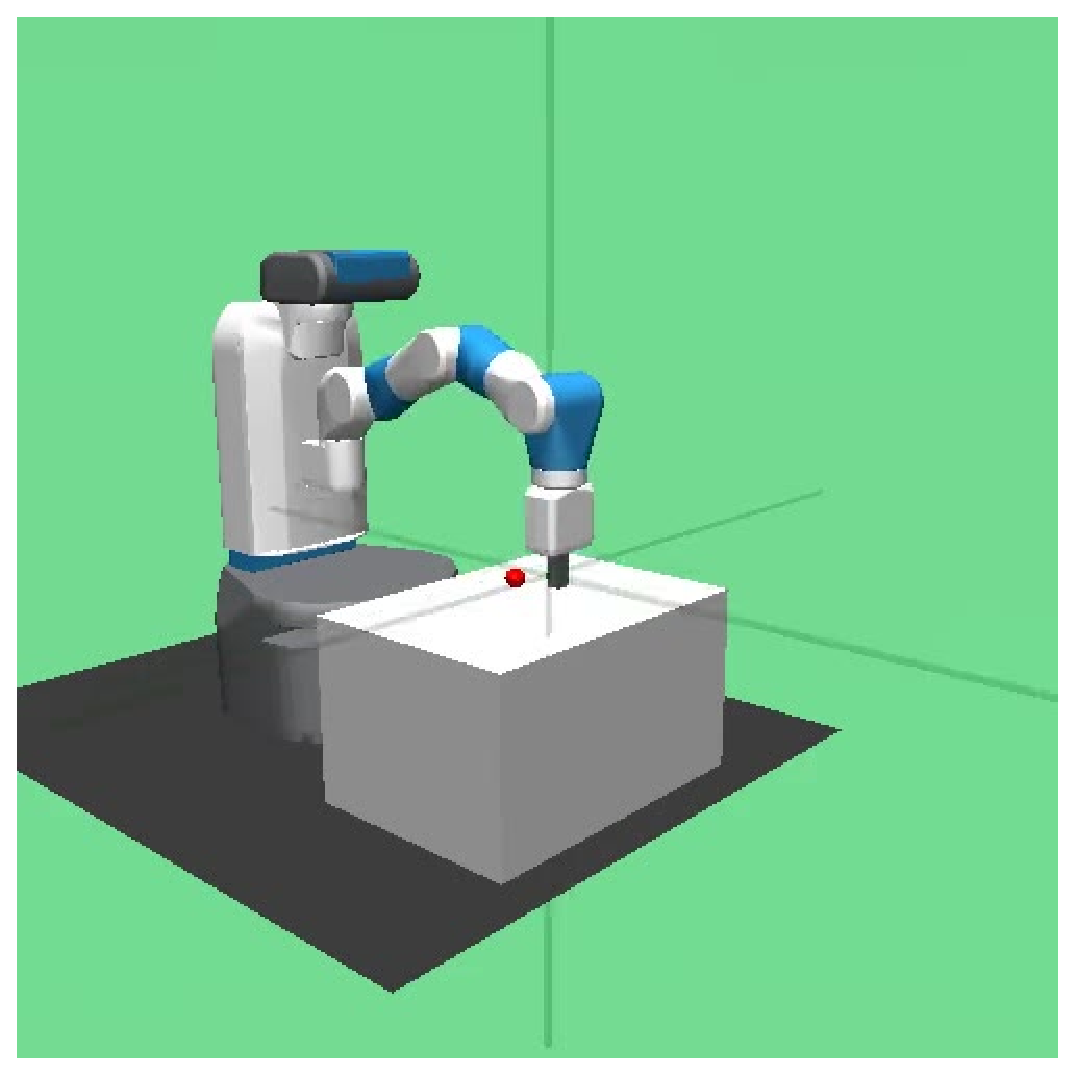
\includegraphics[width=0.3\textwidth]{./fig/fetchreach}
    \label{subfig:fetchreach}
   }
  \subfigure[FetchPush.]
   {
    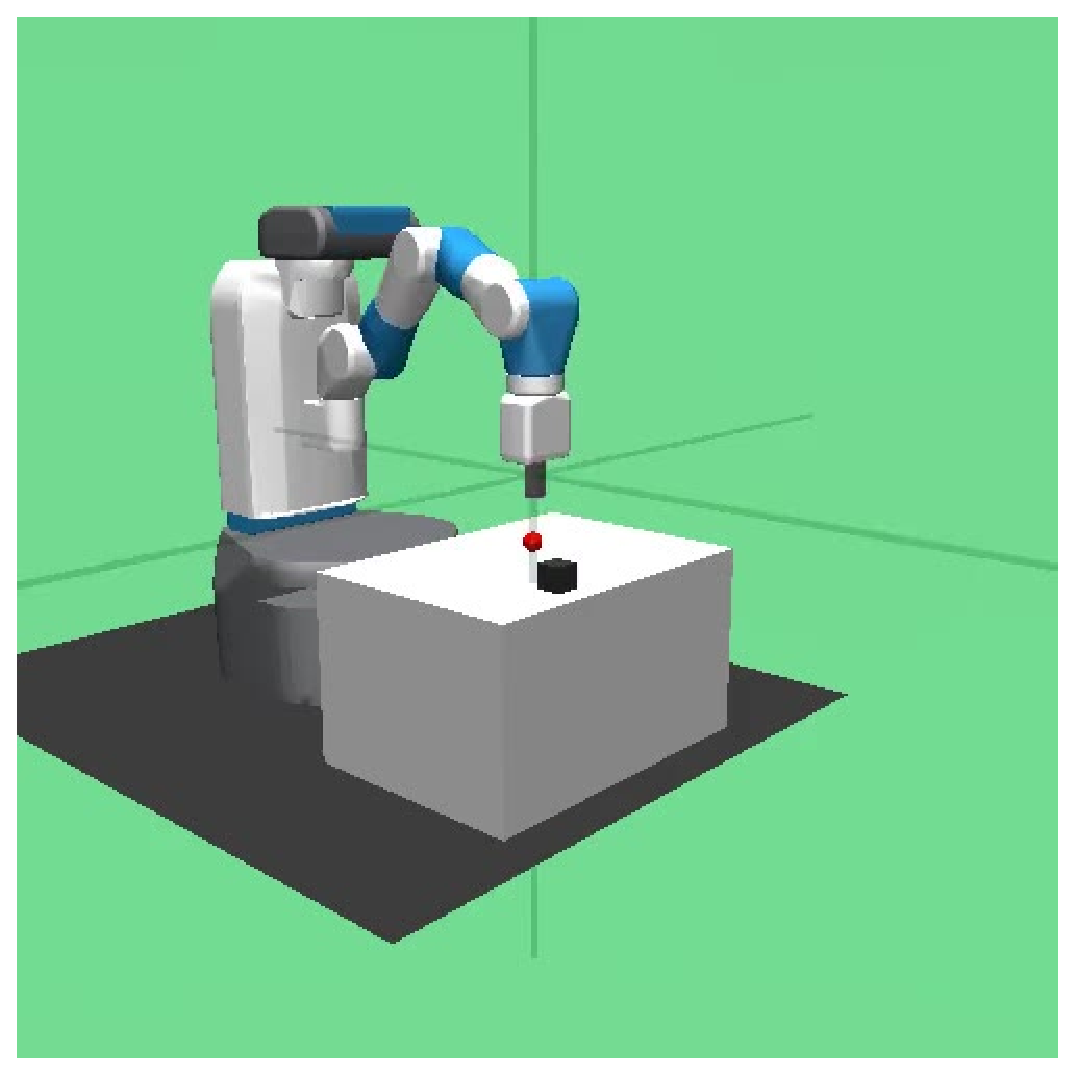
\includegraphics[width=0.3\textwidth]{./fig/fetchpush}
    \label{subfig:fetchpush}
   }
  \subfigure[FetchPickAndPlace.]
   {
    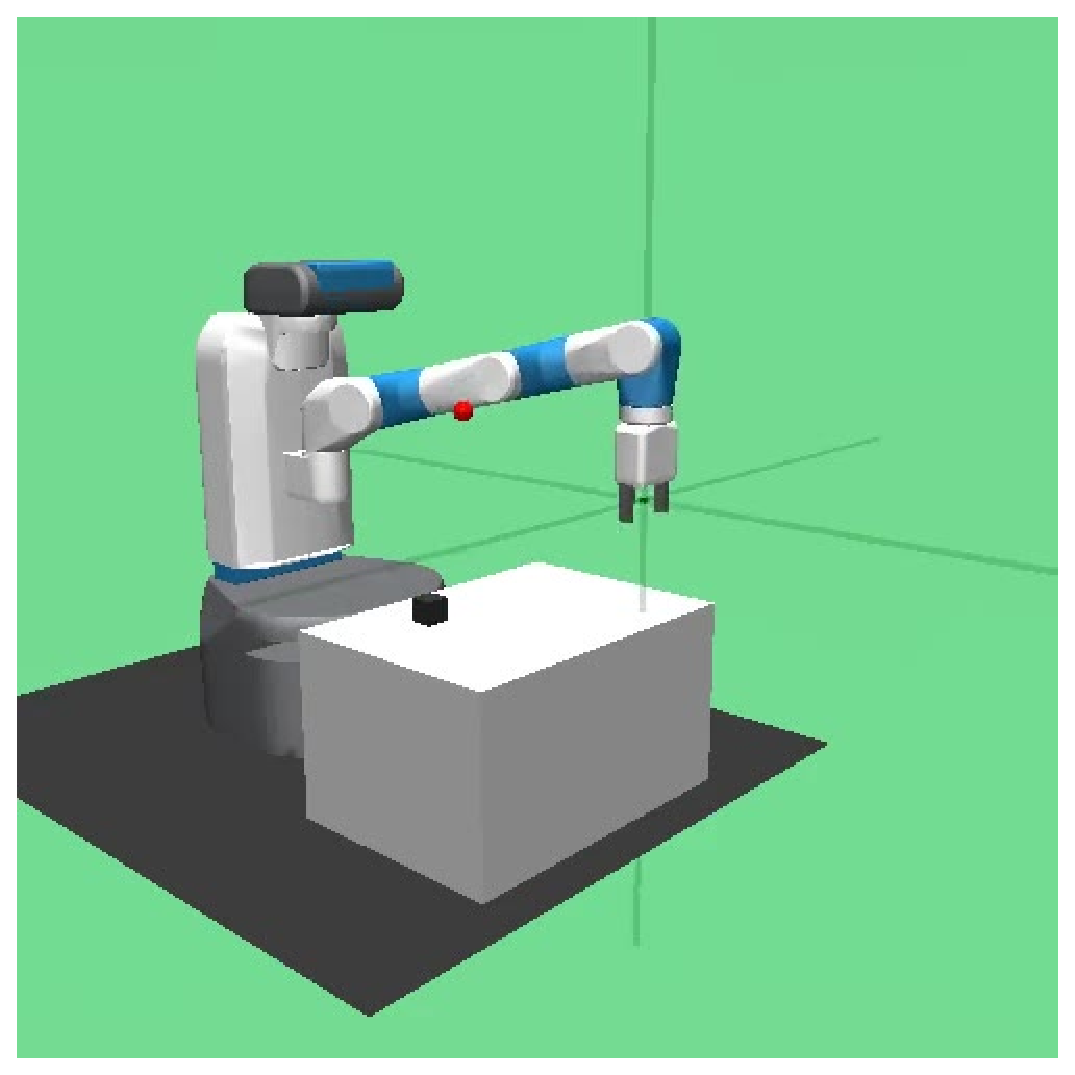
\includegraphics[width=0.3\textwidth]{./fig/fetchpickandplace}
    \label{subfig:fetchpickandplace}
   }
   \captionsetup{width=1\textwidth}
   \caption{Ambientes de manipulação selecionados.}
  \label{fig:fetchenvs}
\end{figure}

Em \textit{FetchReach} (Figura \ref{subfig:fetchreach}) o agente deve posicionar a garra no alvo representado pela esfera vermelha. Em \textit{FecthPickAndPlace} (Figura \ref{subfig:fetchpickandplace}) o agente deve pegar o disco com a garra e posicioná-lo no alvo. Em \textit{FetchPush} (Figura \ref{subfig:fetchpush}) o agente deve empurrar o disco para o alvo.

A recompensa nestes ambientes é considerada, neste trabalho, sendo -1 para todo passo de simulação onde o agente não resolveu a tarefa e 0 quando a tarefa é resolvida. O episódio é limitado a 2048 passos de simulação e é finalizado assim que o agente alcança o objetivo. A observação do ambiente é composta pela posição, rotação e velocidade das juntas do manipulador, assim como posição, rotação e velocidade do disco e a posição do alvo. A ação de um agente neste ambiente é um vetor composto por 4 componentes que representam o torque em cada atuador do manipulador, desde cada junta até a abertura da garra.

% - - - - - - - - - - - - - - - - - - - - - - - - - - - - - - - - - - -

\section{Algoritmo PPO com Motivação Intrínseca}
\label{sec:algoritmo}

O algoritmo utilizado adiciona um passo adicional no funcionamento padrão do PPO descrito em \cite{achiam} e é representado pelo Algoritmo \ref{alg:ppocuriosity} e pela Figura \ref{fig:ppomotivated}. Os passos são descritos com maiores detalhes logo em seguida.

\medskip
\begin{center}
\begin{minipage}{0.92\textwidth}
\begin{algorithm2e}[H]
 \DontPrintSemicolon
 \Entrada{parâmetros da política inicial $\theta_0$, limiar de corte $\epsilon$}
 \Para{$k= 0, 1, 2, ...$} {
    Colete um conjunto de trajetórias $D_k$ com política $\pi_k = \pi(\theta_{k})$ \\
    \Para{cada tupla $(s_t, a_t, r_t, s_{t+1})$ em $D_k$} {
        Calcule o erro do modelo de futuro como mostra a Equação \ref{eqn:curiosityloss} \\
        Calcule a recompensa total $r_t$, como mostra a Equação \ref{eqn:curiosityreward}
    }
    Estime a função de vantagem $A_{t}^{GAE(\gamma, \lambda)}$ \\
    Calcule a atualização da política \\
    \hspace{2cm}$\theta_{k+1} = arg \max_{\theta} L^{CLIP + VF + H}(\theta_k)$ \\
    executando N passos do gradiente ascendente, onde \\
    \hspace{2cm}$L^{CLIP + VF + H}(\theta_k) = \mathop{{}\mathbb{E}}{}_t [L^{CLIP} - L^{VF} + cH(\pi(s_t; \theta))]$ 
 }
\caption{PPO com motivação intrínseca \label{alg:ppocuriosity} }
\end{algorithm2e}
\end{minipage}
\end{center}

Durante a coleta de trajetórias, uma observação $s_t$ do ambiente é passada para o agente a cada passo $t$ de simulação. Essa observação é então alimentada em duas redes neurais: uma rede que calcula a ação $a_t$ a ser tomada, chamada de ator, e uma rede que calcula o valor do estado atual, chamada de crítico. Após a seleção da ação, esta é executada e obtém-se a observação do estado $s_{t+1}$ e a recompensa extrínseca do ambiente. Após o passo de coleta de trajetórias, a recompensa intrínseca é calculada alimentando o modelo de futuro com $(s_t, a_t)$ e calculando o erro $L_F(s_t+1, \hat{s}_{t+1})$. Ao final do episódio o valor da função de vantagem é calculado, os parâmetros do ator são atualizados de acordo com a Equação \ref{eqn:totalloss}, os parâmetros do modelo de futuro são atualizado de acordo com a Equação \ref{eqn:curiosityloss} e os parâmetros do crítico são atualizados de acordo com o erro quadrático médio entre os valores dos estados previstos pela rede e os reais valores obtidos no episódio.

\begin{figure}[ht]
 \centering
  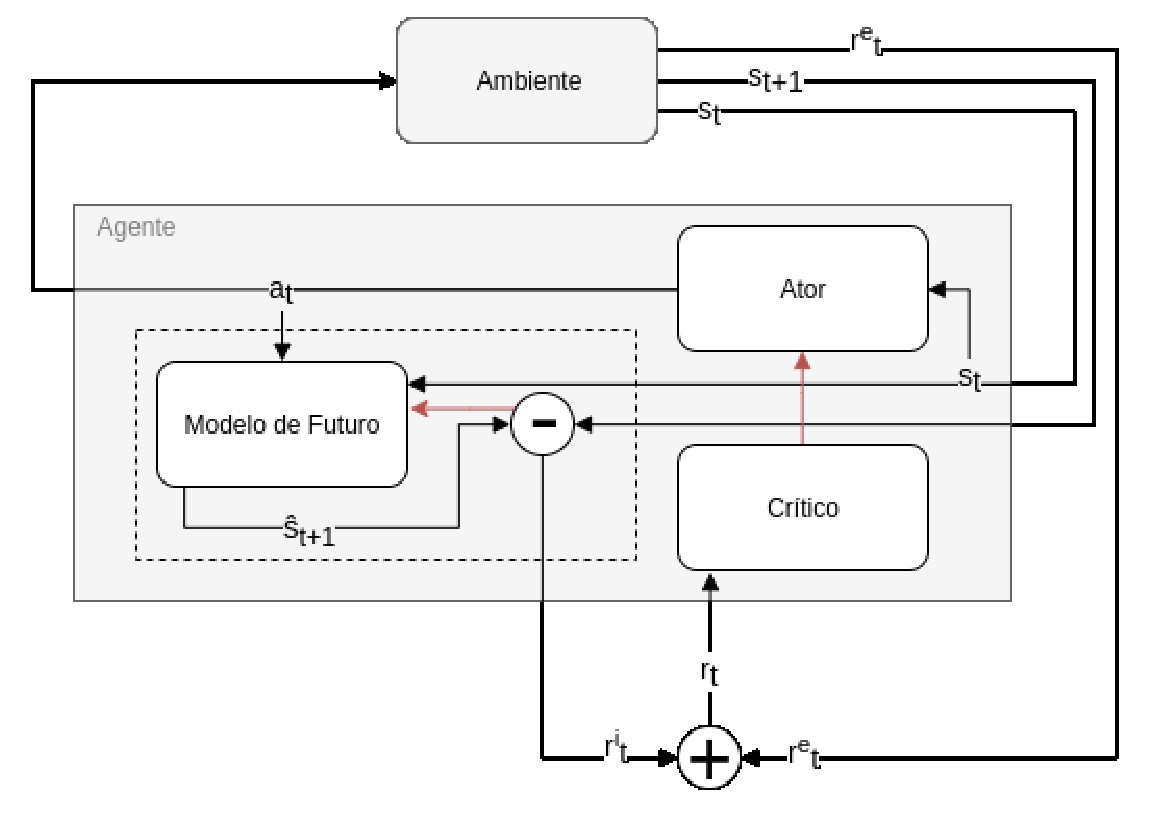
\includegraphics[width=0.70\textwidth]{./fig/ppomotivateddiagram}
  \captionsetup{width=1\textwidth}
  \caption[Diagrama do funcionamento do algoritmo PPO com motivação intrínseca com modelo Ator-Crítico.]{Diagrama do funcionamento do algoritmo PPO com motivação intrínseca com modelo Ator-Crítico. As setas pretas representam os fluxos dos dados no passo de coleta de trajetórias e as setas vermelhas representam o fluxo dos dados no passo de otimização.}
 \label{fig:ppomotivated}
\end{figure}

A rede neural do ator possui duas camadas densas com 128 neurônios cada e função de ativação ReLU, uma terceira camada densa com 15 neurônios e função de ativação TanH e uma camada densa final que tem por objetivo determinar a média $\mu$ da distribuição de probabilidades da saída. O desvio padrão $\sigma$ da distribuição é determinada por parâmetros aprendidos pelo próprio modelo e tende a ser controlado a fim de manter a entropia da distribuição alta enquanto for possível \cite{williamspeng}. A ação do agente é selecionada fazendo a amostragem da distribuição $N(\mu, \sigma^2)$. A rede neural do crítico possui uma topologia semelhante a do ator nas duas primeiras camadas mas sua camada de saída possui apenas um neurônio. A configuração detalhada dos hiperparâmetros do algoritmo utilizado nos experimentos pode ser conferida no Apêndice \ref{apend:1}.

% - - - - - - - - - - - - - - - - - - - - - - - - - - - - - - - - - - -

\section{Testes}
\label{sec:testes}

Os testes são executados de forma a analisar o impacto da motivação intrínseca no aprendizado por reforço em ambientes de manipulação robótica com recompensa esparsa. Para isso, o treinamento do agente é executado nas mesmas condições em dois testes, onde no primeiro a recompensa intrínseca é adicionada à recompensa total e na segunda somente a recompensa extrínseca é transmitida. Para cada teste, o agente foi treinado no ambiente \textit{FetchReach} por 10 milhões de iterações iterações e nos ambientes \textit{FetchPush} e \textit{FetchPickAndPlace} por 30 milhões de iterações. Os testes foram executados paralelamente em seis máquinas com dez núcleos de processamento cada e sem GPUs, resultando em um tempo de treinamento total de aproximadamente oito horas. Os resultados são obtidos durante o processo de treinamento através da ferramenta Tensorboard\footnote{Disponível em \url{https://www.tensorflow.org/tensorboard/get\_started}}.

Como métrica de desempenho é analisada a porcentagem de sucessos em cada lote de avaliações durante o treinamento de cada tarefa, assim como a recompensa intrínseca média, a entropia da política e a divergência KL entre as políticas de antes e depois de uma atualização de parâmetros. A taxa de sucesso mostra a eficiência do algoritmo em alcançar o objetivo e se isso ocorre de forma consistente. A recompensa intrínseca mostra como o modelo de futuro se comporta ao se deparar com os diversos estados em que o agente se encontra durante o treino e testa sua capacidade de predição, ou seja, o entendimento da dinâmica do ambiente. Picos no gráfico de recompensa intrínseca podem indicar aumento do interesse do agente sobre alguma situação específica que modificou o padrão das observações do ambiente de forma significativa. A entropia da política indica quão conservador o agente é em relação a probabilidade de escolha entre as ações, ou seja, se o mesmo permite que diferentes sequências de ações sejam tomadas para atingir seus objetivos. Altos valores de entropia da política podem indicar boas capacidades de generalização, uma vez que mostra que o agente não só simplesmente "decorou" uma sequência específica de ações que resolve o objetivo \cite{williamspeng}. A divergência KL mostra o ritmo no qual a política se modifica entre as atualizações. Esse ritmo tende a ser alto em fases do treinamento em que o agente está modificando significativamente sua política e pode estar relacionado com quedas ou aumentos em sua taxa de sucesso.

Como hipótese, é esperado que o agente com recompensa intrínseca se saia melhor que o algoritmo sem a mesma, refletindo na razão de sucessos máxima de ambos e na velocidade em que se estabilizam nesta métrica. Além disso, espera-se picos de recompensa intrínseca quando mudanças de comportamento do agente influenciam diferentes aspectos da observação no ambiente.
\chapter{Resultados}
\label{cap:resultados}

Neste Capítulo são descritos os resultados obtidos da execução dos testes descritos no capítulo anterior. Para cada ambiente de teste, o agente foi treinado uma vez utilizando o módulo de motivação intrínseca e uma vez sem utilizá-lo pelo mesmo número de iterações. Na análise, nos referimos ao agente do segundo treinamento como algoritmo, ou agente, \textit{baseline}. Dizemos também que o algoritmo "convergiu" quando sua razão de sucessos se torna satisfatória. Em todos os gráficos, o eixo horizontal representa o número de iterações, as linhas em vermelho indicam o uso do algoritmo PPO com motivação intrínseca, ou curiosidade, e as linhas azuis indicam o uso algoritmo PPO \textit{baseline}. Nos gráficos de recompensa intrínseca e de divergência KL as linhas foram suavizadas\footnote{O filtro de Savitzky-Golay, implementado pela biblioteca SciPy \cite{scipy}, foi utilizado com uma janela de tamanho 31 e ordem polinomial 3.} para melhor compreensão. Os resultados foram agrupados de acordo com os ambientes treinados e uma análise geral é feita ao final deste Capítulo.

% - - - - - - - - - - - - - - - - - - - - - - - - - - - - - - - - - - -
\section{\textit{FetchReach}}
\label{sec:reach}

\begin{figure}[h!]
 \centering
  \subfigure[Início do episódio.]
   {
    \includegraphics[width=0.3\textwidth]{./fig/reach_ex_1}
    \label{subfig:reach_ex_1}
   }
  \subfigure[Episódio em progresso.]
   {
    \includegraphics[width=0.3\textwidth]{./fig/reach_ex_2}
    \label{subfig:reach_ex_2}
   }
  \subfigure[Próximo do fim do episódio.]
   {
    \includegraphics[width=0.3\textwidth]{./fig/reach_ex_3}
    \label{subfig:reach_ex_3}
   }
   \captionsetup{width=1\textwidth}
   \caption{Progresso do agente treinado com curiosidade no ambiente FetchReach.}
  \label{fig:reach_ex}
\end{figure}

No ambiente \textit{FetchReach}, ambos os algoritmos alcançaram 100\% de sucesso em menos de dois milhões de passos de simulação. A Figura \ref{fig:reach_ex} mostra o agente treinado com módulo de curiosidade em alguns passos de simulação. É interessante notar o decaimento do valor da recompensa intrínseca (Figura \ref{subfig:reach_int}) em um ritmo semelhante ao aumento da razão de sucessos do algoritmo PPO com módulo de curiosidade (Figura \ref{subfig:reach_suc}). Este fenômeno pode indicar o aprendizado da dinâmica do ambiente por parte do agente, ou seja, a medida em que o agente descobre como suas ações influenciam o ambiente e, consequentemente, mais próximo está de seu objetivo, menos surpreso com os novos estados ele fica.

\begin{figure}[h!]
 \centering
  \subfigure[Razão de sucessos.]
   {
    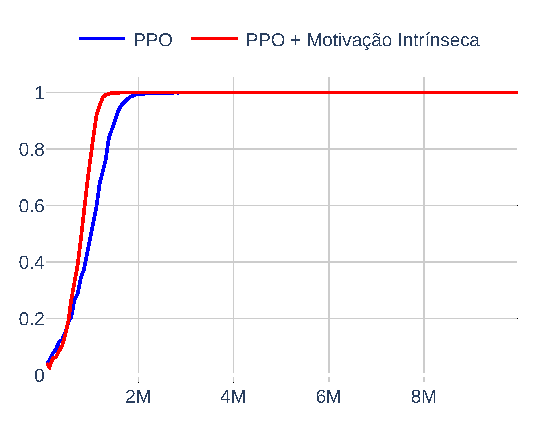
\includegraphics[width=0.45\textwidth]{./fig/reach}
    \label{subfig:reach_suc}
   }
  \subfigure[Recompensa intrínseca média.]
   {
    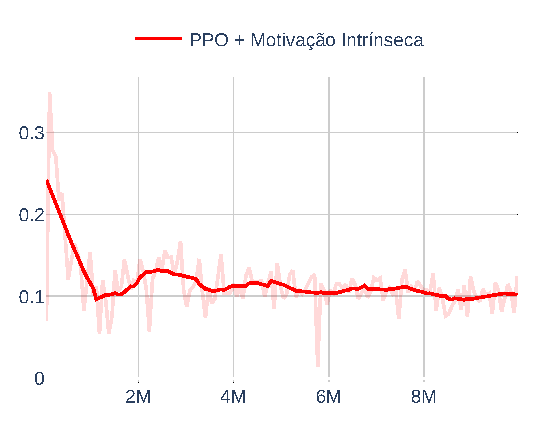
\includegraphics[width=0.45\textwidth]{./fig/reach_int}
    \label{subfig:reach_int}
   }
  \subfigure[Entropia da política.]
   {
    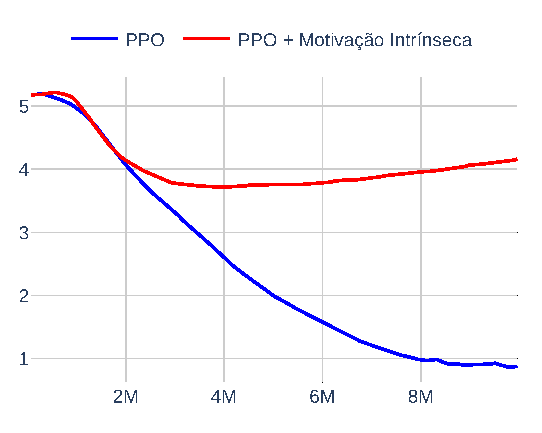
\includegraphics[width=0.45\textwidth]{./fig/reach_ent}
    \label{subfig:reach_ent}
   }
  \subfigure[Divergência KL entre as políticas.]
   {
    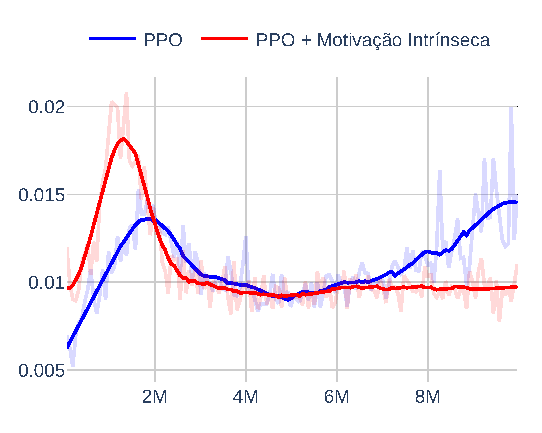
\includegraphics[width=0.45\textwidth]{./fig/reach_kl}
    \label{subfig:reach_kl}
   }
   \caption{Estatísticas para o ambiente FetchReach.}
  \label{fig:reach}
\end{figure}


Outra análise que pode ser feita neste ambiente é em relação aos gráficos de entropia (Figura \ref{subfig:reach_ent}) e divergência KL (Figura \ref{subfig:reach_kl}). A entropia da política do agente com módulo de curiosidade tende a se manter alta mesmo após a convergência do algoritmo, enquanto que o agente \textit{baseline} diminui sua entropia se tornando cada vez mais determinístico. Na prática, vemos que o agente com curiosidade se mantém com altos níveis de exploração, possibilitando que melhores sequências de ações para alcançar o objetivo proposto sejam encontradas. Pode-se observar também pelo gráfico de divergência KL que após a convergência a política do agente com curiosidade tende sofrer poucas modificações em relação à política do agente \textit{baseline}. Este comportamento reforça ainda mais a hipótese de que a dinâmica do ambiente foi aprendida pelo agente com curiosidade, fazendo com que a recompensa intrínseca seja muito menor e as alterações na política sejam mínimas.

% - - - - - - - - - - - - - - - - - - - - - - - - - - - - - - - - - - -

\section{\textit{FetchPush}}
\label{sec:push}

No ambiente \textit{FetchPush} o algoritmo PPO original não conseguiu resolver a tarefa durante o treinamento, como mostra o gráfico da Figura \ref{subfig:push_suc}. Uma explicação é a quantidade de ações em sequência necessárias para alcançar o objetivo, tornando baixa a chance disso ocorrer por acaso. O PPO com módulo de curiosidade, no entanto, pode aproveitar o incentivo que recebe ao explorar as posições do próprio manipulador e, o mais impactante, o comportamento do bloco quando o atinge por acaso. Como a posição, rotação e velocidades do bloco fazem parte da observação do agente e o modelo de futuro não conhece a dinâmica do bloco no início do treinamento, esbarrar no mesmo faz com que o erro de predição aumente de forma significativa. Como o erro de predição é diretamente proporcional à recompensa intrínseca do agente, este se torna consideravelmente interessado em jogar o bloco de um lado para o outro, eventualmente alcançando o objetivo. Quando este processo ocorre, observa-se um pico no gráfico de recompensa intrínseca (Figura \ref{subfig:push_int}) e logo em seguida um aumento na taxa de sucesso (Figura \ref{subfig:push_suc}).

\begin{figure}[h!]
 \centering
  \subfigure[Início do episódio.]
   {
    \includegraphics[width=0.3\textwidth]{./fig/push_ex_1}
    \label{subfig:push_ex_1}
   }
  \subfigure[Episódio em progresso.]
   {
    \includegraphics[width=0.3\textwidth]{./fig/push_ex_2}
    \label{subfig:push_ex_2}
   }
  \subfigure[Fim do episódio.]
   {
    \includegraphics[width=0.3\textwidth]{./fig/push_ex_3}
    \label{subfig:push_ex_3}
   }
   \caption{Progresso do agente treinado com curiosidade no ambiente FetchPush.}
  \label{fig:push_ex}
\end{figure}

\begin{figure}[h!]
 \centering
  \subfigure[Razão de sucessos.]
   {
    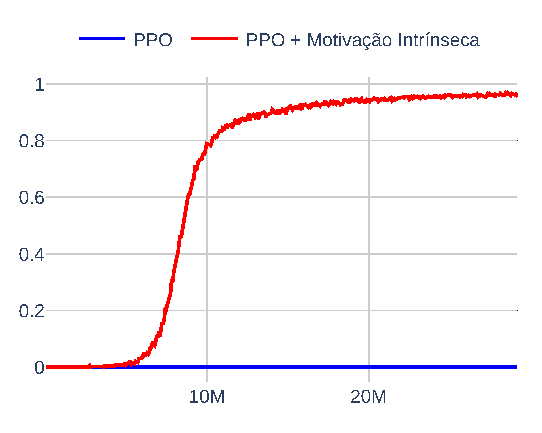
\includegraphics[width=0.45\textwidth]{./fig/push}
    \label{subfig:push_suc}
   }
  \subfigure[Recompensa intrínseca média.]
   {
    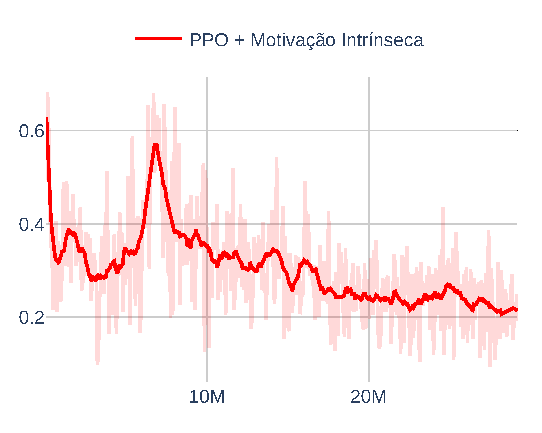
\includegraphics[width=0.45\textwidth]{./fig/push_int}
    \label{subfig:push_int}
   }
  \subfigure[Entropia da política.]
   {
    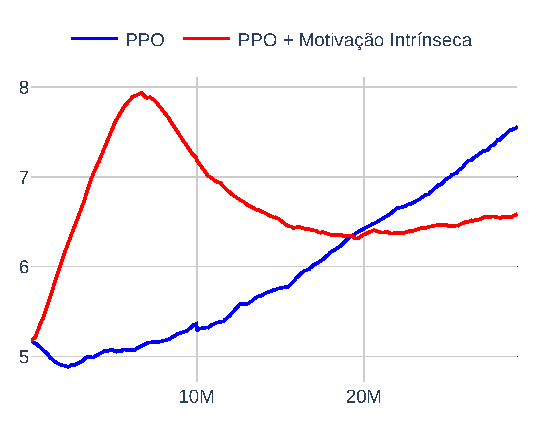
\includegraphics[width=0.45\textwidth]{./fig/push_ent}
    \label{subfig:push_ent}
   }
  \subfigure[Divergência KL entre as políticas.]
   {
    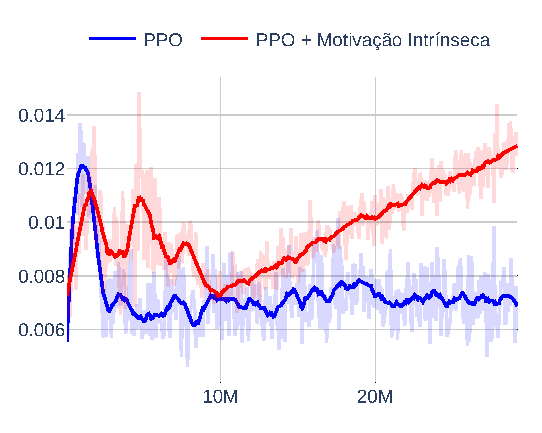
\includegraphics[width=0.45\textwidth]{./fig/push_kl}
    \label{subfig:push_kl}
   }
   \caption{Estatísticas para o ambiente FetchPush.}
  \label{fig:push}
\end{figure}

O gráfico de divergência KL (Figura \ref{subfig:push_kl}) mostra como a política do agente com curiosidade é modificada gradativamente durante o treino, mesmo após a convergência. Como a razão de sucessos ao final do treinamento foi de 96\%, como mostra a Tabela \ref{tab:taxasuc}, e a recompensa intrínseca possuía um valor considerável, acredita-se que o agente poderia melhorar sua política ainda mais. Além disso, o gráfico da Figura \ref{subfig:push_ent} mostra como a entropia da política do agente com curiosidade possui um pico logo no início do treinamento, possivelmente motivado pela recompensa intrínseca, e como a mesma se estabiliza em valores altos após a convergência. O agente \textit{baseline}, por outro lado, não recebendo sinais de como modificar sua política opta por aumentar a entropia das distribuições das ações, reforçando seu comportamento exploratório. Além disso, é possível ver que a divergência KL entre as políticas do agente \textit{baseline} se mantém relativamente constante. Um exemplo de episódio em que o agente treinado com curiosidade consegue resolver a tarefa é mostrado na Figura \ref{fig:push_ex}.

% - - - - - - - - - - - - - - - - - - - - - - - - - - - - - - - - - - -

\section{\textit{FetchPickAndPlace}}
\label{sec:pick}

\begin{figure}[h!]
 \centering
  \subfigure[Início do episódio.]
   {
    \includegraphics[width=0.3\textwidth]{./fig/pick_ex_1}
    \label{subfig:pick_ex_1}
   }
  \subfigure[Episódio em progresso.]
   {
    \includegraphics[width=0.3\textwidth]{./fig/pick_ex_2}
    \label{subfig:pick_ex_2}
   }
  \subfigure[Fim do episódio.]
   {
    \includegraphics[width=0.3\textwidth]{./fig/pick_ex_3}
    \label{subfig:pick_ex_3}
   }
   \captionsetup{width=1\textwidth}
   \caption{Progresso do agente treinado com curiosidade no ambiente FetchPickAndPlace.}
  \label{fig:pick_ex}
\end{figure}

Neste ambiente, assim como em \textit{FetchPush}, o algoritmo PPO original não é capaz de realizar a tarefa durante o treinamento (Figura \ref{subfig:pick_suc}) pelos mesmos motivos. Neste ambiente o desafio é ainda maior, pois uma grande quantidade de ações extremamente específicas devem ser executadas para alcançar o objetivo. Para o PPO com módulo de curiosidade, porém, a tarefa ainda é factível. O agente é recompensado já em poucas iterações após o início do treino ao interagir com o bloco, sendo encorajado a manipulá-lo uma vez que sua posição, rotação e velocidades fazem parte de sua observação, o que influencia em sua recompensa intrínseca (Figura \ref{subfig:pick_int}). Neste caso nota-se também que sua evolução é um processo mais lento, cerca de 15 milhões de iterações para que o agente alcance mais de 85\% de sucesso.

\begin{figure}[h!]
 \centering
  \subfigure[Razão de sucessos.]
   {
    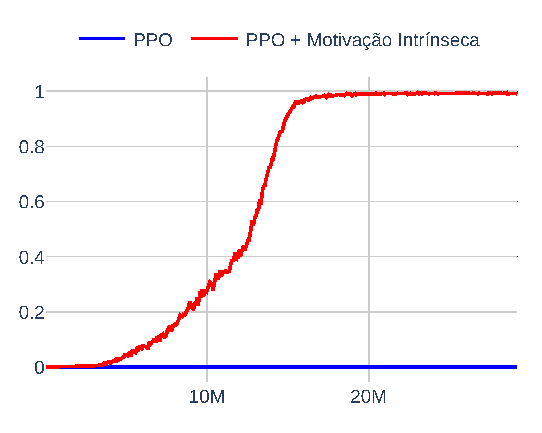
\includegraphics[width=0.45\textwidth]{./fig/pick}
    \label{subfig:pick_suc}
   }
  \subfigure[Recompensa intrínseca média.]
   {
    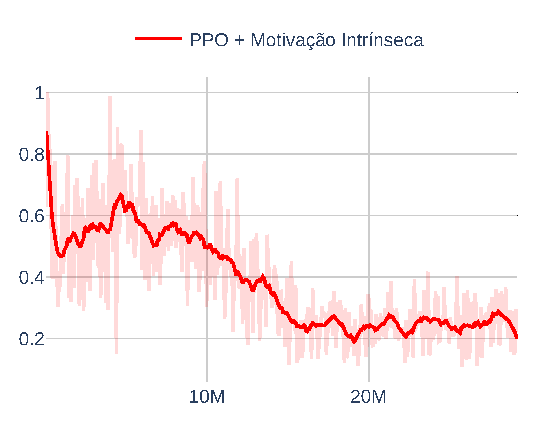
\includegraphics[width=0.45\textwidth]{./fig/pick_int}
    \label{subfig:pick_int}
   }
  \subfigure[Entropia da política.]
   {
    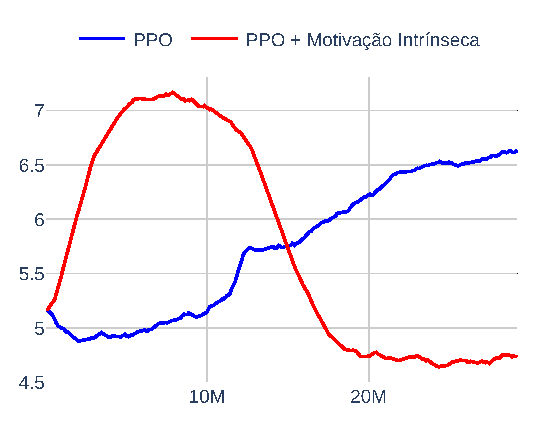
\includegraphics[width=0.45\textwidth]{./fig/pick_ent}
    \label{subfig:pick_ent}
   }
  \subfigure[Divergência KL entre as políticas.]
   {
    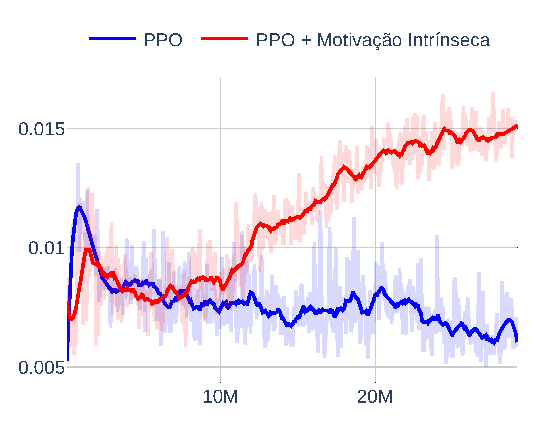
\includegraphics[width=0.45\textwidth]{./fig/pick_kl}
    \label{subfig:pick_kl}
   }
   \caption{Estatísticas para o ambiente FetchPickAndPlace.}
  \label{fig:pick}
\end{figure}

Mais uma vez, há um pico no gráfico de recompensa intrínseca pouco antes da taxa de sucesso do agente começar a subir. A curiosidade do agente diminui poucas iterações após a convergência, uma vez que a dinâmica do ambiente não trás mais tantas novidades. Além disso, observa-se o mesmo comportamento nos gráficos de entropia (Figura \ref{subfig:pick_ent}) e divergência KL entre políticas (Figura \ref{subfig:pick_kl}) se comparado com o ambiente \textit{FetchPush}. O interessante a se notar, porém, é quão conservadora em relação a uniformidade das probabilidades de ações o agente se tornou neste ambiente, como mostra o gráfico de entropia. Esse comportamento é esperado pois o agente deve sempre abrir a garra para segurar o bloco e evitar soltá-lo, uma vez que o mesmo pode cair da mesa, fora de seu alcance. A Figura \ref{fig:pick_ex} mostra o agente treinado com curiosidade resolvendo a tarefa proposta.

% - - - - - - - - - - - - - - - - - - - - - - - - - - - - - - - - - - -

\section{Considerações Gerais}
\label{sec:resgerais}

Em geral, o algoritmo com módulo de curiosidade foi capaz de resolver as tarefas de todos os ambientes, como mostra a Tabela \ref{tab:taxasuc}. É interessante notar que a taxa de sucesso no ambiente \textit{FetchPickAndPlace} é maior que a taxa de sucesso no ambiente \textit{FetchPush}. Isso acontece pois em algumas avaliações no ambiente \textit{FetchPush} o manipulador pode jogar o bloco para fora da mesa, impossibilitando o agente de completar sua tarefa. Em \textit{FetchPickAndPlace} a garra do manipulador robótico raramente solta o bloco uma vez que conseguiu agarrá-lo. Após segurar o bloco, basta que o agente se comporte como em \textit{FetchReach}, o que é uma tarefa simples.

\begin{table*}[h!]
\centering
\captionsetup{width=1\textwidth}
\caption{Razão de sucesso dos algoritmos em cada ambiente de teste.}
\label{tab:taxasuc} 
\begin{tabular}{|c|c|c|c|c|c|c|}
\hline Algoritmo & FetchReach & FetchPush & FetchPickAndPlace \\ 
\hline PPO & 100\% & 0\% & 0\%\\ 
\hline PPO + Motivação Intrínseca & 100\% & 96\% & 99\%\\ 
\hline 
\end{tabular} 
\end{table*}
\chapter{Conclusões}
\label{cap:conclusao}

Neste trabalho, foi apresentada uma alternativa para o treinamento de agentes de aprendizado por reforço em ambientes com recompensa esparsa ou inexistente. Foi demonstrado que agentes utilizando a técnica de motivação intrínseca, ou curiosidade, conseguem resolver tarefas consideravelmente difíceis do domínio da robótica.

No Capítulo \ref{cap:intro} foi exposto o problema da programação de comportamentos complexos em robôs e algumas soluções utilizando técnicas de aprendizado por reforço. Foi apresentado também como comumente estes problemas são formulados para o treinamento de agentes e o desafio do aprendizado em ambientes com recompensa esparsa, que é a motivação deste trabalho. A proposta do uso de um módulo de motivação intrínseca, inspirada por trabalhos recentes na área de aprendizado por reforço, também foi descrita.

No Capítulo \ref{cap:fundamentacao} foram apresentados os fundamentos teóricos que foram base para a preparação e execução dos experimentos. Primeiramente, foram definidos os conceitos de aprendizado de máquina, redes neurais e aprendizado por reforço. Os fundamentos do algoritmo utilizado como base para este trabalho, o PPO, foram apresentados em seguida, assim como o funcionamento do módulo de motivação intrínseca para exploração, que foi o foco deste estudo.

No Capítulo \ref{cap:metodologia} foram definidos os ambientes de \textit{benchmark} selecionados e seu funcionamento foi descrito. O funcionamento completo do algoritmo utilizado e a comunicação entre os modelos de predição de valor do estado, da política e de predição do estado futuro também foram apresentados. Em seguida, a metodologia para os experimentos executados foi definida. Para a demonstração do impacto do módulo de curiosidade no aprendizado, o mesmo algoritmo com os mesmos hiperparâmetros foi executado duas vezes em cada ambiente - uma vez com o módulo de curiosidade e outra vez sem o mesmo.

Os resultados, apresentados no Capítulo \ref{cap:resultados}, demonstram um comportamento exploratório capaz de executar complexas sequências de ações por parte do algoritmo proposto, permitindo-o alcançar o objetivo em todos os ambientes em que foi testado. Os gráficos apresentados demonstram também a tendência do agente a manter políticas exploratórias mesmo alcançando o objetivo geral de cada tarefa proposta. Essas tendências indicam um comportamento possivelmente generalista que pode ser útil para aplicações em problemas que requerem uma abordagem multitarefa ou até de meta-aprendizado.

Nesse contexto, são propostas algumas direções para trabalhos futuros. Primeiramente, o impacto da motivação intrínseca em ambientes multitarefa e de meta-aprendizado pode ser analisado. \textit{Benchmarks} propostos recentemente \cite{metaworld} se mostraram robustos para a avaliação dessas capacidades. Além disso, o estudo da capacidade de generalização do algoritmo para ambientes de teste diferentes dos quais o agente foi treinado é uma importante métrica a ser avaliada. Outras ideias para futuros trabalhos envolvem a aplicação de motivação intrínseca para controle em sistemas complexos e de característica hierárquica, assim como sua aplicação em sistemas de aprendizado multi-agente. Por fim, o uso de curiosidade para aprendizado de controle a partir de píxeis pode ser explorado, dado o sucesso da aplicação desta configuração em jogos \cite{curiositylarge} e pela facilidade e viabilidade do uso de câmeras em robôs reais.

%------------------------------------------------------------ BIBLIOGRAFIA %
\cleardoublepage
%\nocite{*} %%% Retire esta linha para gerar a bibliografia com apenas as
           %%% referências usadas no seu texto!
\arial
\bibliography{modelo-tese} %%% Nomes dos seus arquivos .bib
\label{ref-bib}

%--------------------------------------------------------------- APÊNDICES %
\apendices

\chapter{Hiperparâmetros}
\label{apend:1}

\begin{table*}[ht]
\centering
\caption{Hiperparâmetros para o algoritmo PPO e módulo de motivação intrínseca.}
\label{tab:hiperparameters} 
\begin{tabular}{|c|c|}
\hline Hiperparâmetro & Valor \\
\hline Iterações (em cada ambiente) & $3x10^7$ \\
\hline Neurônios nas camadas escondidas & $128$ \\ 
\hline Taxa de aprendizado do modelo de valor & $10^{-4}$ \\
\hline Taxa de aprendizado do modelo da política & $10^{-5}$ \\
\hline Taxa de aprendizado do modelo de futuro & $10^{-5}$ \\
\hline Coeficiente de entropia & $0.01$ \\ 
\hline Recompensa intrínseca máxima & $1$ \\
\hline Tamanho do episódio & $2048$ \\ 
\hline Tamanho do lote & $32$ \\ 
\hline Épocas & $10$ \\ 
\hline $\gamma$ & $0.95$ \\ 
\hline $\epsilon$ (PPO) & $0.3$ \\
\hline $\lambda$ (GAE) & $0.95$ \\
\hline $\eta$ (recompensa intrínseca) & $1$ \\
\hline Otimizador & Adam \\
\hline 
\end{tabular} 
\end{table*}
%\chapter{Exemplo de Outro Apêndice}
\label{apend:2}
Texto do Apêndice~\ref{apend:2}.

Apêndices são iniciados com o comando \verb|\apendices|.
Apêndices são iniciados com o comando \verb|\apendices|.
Apêndices são iniciados com o comando \verb|\apendices|.
Apêndices são iniciados com o comando \verb|\apendices|.
Apêndices são iniciados com o comando \verb|\apendices|.
Apêndices são iniciados com o comando \verb|\apendices|.
Apêndices são iniciados com o comando \verb|\apendices|.
Apêndices são iniciados com o comando \verb|\apendices|.
Apêndices são iniciados com o comando \verb|\apendices|.
Apêndices são iniciados com o comando \verb|\apendices|.
Apêndices são iniciados com o comando \verb|\apendices|.
Apêndices são iniciados com o comando \verb|\apendices|.
Apêndices são iniciados com o comando \verb|\apendices|.
Apêndices são iniciados com o comando \verb|\apendices|.
Apêndices são iniciados com o comando \verb|\apendices|.
Apêndices são iniciados com o comando \verb|\apendices|.

Apêndices são iniciados com o comando \verb|\apendices|.
Apêndices são iniciados com o comando \verb|\apendices|.
Apêndices são iniciados com o comando \verb|\apendices|.
Apêndices são iniciados com o comando \verb|\apendices|.
Apêndices são iniciados com o comando \verb|\apendices|.
Apêndices são iniciados com o comando \verb|\apendices|.
Apêndices são iniciados com o comando \verb|\apendices|.
Apêndices são iniciados com o comando \verb|\apendices|.
Apêndices são iniciados com o comando \verb|\apendices|.
Apêndices são iniciados com o comando \verb|\apendices|.
Apêndices são iniciados com o comando \verb|\apendices|.
Apêndices são iniciados com o comando \verb|\apendices|.

Apêndices são iniciados com o comando \verb|\apendices|.
Apêndices são iniciados com o comando \verb|\apendices|.
Apêndices são iniciados com o comando \verb|\apendices|.
Apêndices são iniciados com o comando \verb|\apendices|.
Apêndices são iniciados com o comando \verb|\apendices|.
Apêndices são iniciados com o comando \verb|\apendices|.
Apêndices são iniciados com o comando \verb|\apendices|.
Apêndices são iniciados com o comando \verb|\apendices|.
Apêndices são iniciados com o comando \verb|\apendices|.
Apêndices são iniciados com o comando \verb|\apendices|.
Apêndices são iniciados com o comando \verb|\apendices|.
Apêndices são iniciados com o comando \verb|\apendices|.
Apêndices são iniciados com o comando \verb|\apendices|.
Apêndices são iniciados com o comando \verb|\apendices|.

Apêndices são iniciados com o comando \verb|\apendices|.
Apêndices são iniciados com o comando \verb|\apendices|.
Apêndices são iniciados com o comando \verb|\apendices|.
Apêndices são iniciados com o comando \verb|\apendices|.
Apêndices são iniciados com o comando \verb|\apendices|.
Apêndices são iniciados com o comando \verb|\apendices|.
Apêndices são iniciados com o comando \verb|\apendices|.
Apêndices são iniciados com o comando \verb|\apendices|.
Apêndices são iniciados com o comando \verb|\apendices|.
Apêndices são iniciados com o comando \verb|\apendices|.
Apêndices são iniciados com o comando \verb|\apendices|.
Apêndices são iniciados com o comando \verb|\apendices|.
Apêndices são iniciados com o comando \verb|\apendices|.
Apêndices são iniciados com o comando \verb|\apendices|.

Apêndices são iniciados com o comando \verb|\apendices|.
Apêndices são iniciados com o comando \verb|\apendices|.
Apêndices são iniciados com o comando \verb|\apendices|.
Apêndices são iniciados com o comando \verb|\apendices|.
Apêndices são iniciados com o comando \verb|\apendices|.
Apêndices são iniciados com o comando \verb|\apendices|.
Apêndices são iniciados com o comando \verb|\apendices|.
Apêndices são iniciados com o comando \verb|\apendices|.
Apêndices são iniciados com o comando \verb|\apendices|.
Apêndices são iniciados com o comando \verb|\apendices|.
Apêndices são iniciados com o comando \verb|\apendices|.
Apêndices são iniciados com o comando \verb|\apendices|.
Apêndices são iniciados com o comando \verb|\apendices|.
Apêndices são iniciados com o comando \verb|\apendices|.

Apêndices são iniciados com o comando \verb|\apendices|.
Apêndices são iniciados com o comando \verb|\apendices|.
Apêndices são iniciados com o comando \verb|\apendices|.
Apêndices são iniciados com o comando \verb|\apendices|.
Apêndices são iniciados com o comando \verb|\apendices|.
Apêndices são iniciados com o comando \verb|\apendices|.
Apêndices são iniciados com o comando \verb|\apendices|.
Apêndices são iniciados com o comando \verb|\apendices|.
Apêndices são iniciados com o comando \verb|\apendices|.
Apêndices são iniciados com o comando \verb|\apendices|.
Apêndices são iniciados com o comando \verb|\apendices|.
Apêndices são iniciados com o comando \verb|\apendices|.
Apêndices são iniciados com o comando \verb|\apendices|.
Apêndices são iniciados com o comando \verb|\apendices|.

Apêndices são iniciados com o comando \verb|\apendices|.
Apêndices são iniciados com o comando \verb|\apendices|.
Apêndices são iniciados com o comando \verb|\apendices|.
Apêndices são iniciados com o comando \verb|\apendices|.
Apêndices são iniciados com o comando \verb|\apendices|.
Apêndices são iniciados com o comando \verb|\apendices|.
Apêndices são iniciados com o comando \verb|\apendices|.
Apêndices são iniciados com o comando \verb|\apendices|.
Apêndices são iniciados com o comando \verb|\apendices|.
Apêndices são iniciados com o comando \verb|\apendices|.
Apêndices são iniciados com o comando \verb|\apendices|.
Apêndices são iniciados com o comando \verb|\apendices|.
Apêndices são iniciados com o comando \verb|\apendices|.
Apêndices são iniciados com o comando \verb|\apendices|.

Apêndices são iniciados com o comando \verb|\apendices|.
Apêndices são iniciados com o comando \verb|\apendices|.
Apêndices são iniciados com o comando \verb|\apendices|.
Apêndices são iniciados com o comando \verb|\apendices|.
Apêndices são iniciados com o comando \verb|\apendices|.
Apêndices são iniciados com o comando \verb|\apendices|.
Apêndices são iniciados com o comando \verb|\apendices|.
Apêndices são iniciados com o comando \verb|\apendices|.
Apêndices são iniciados com o comando \verb|\apendices|.
Apêndices são iniciados com o comando \verb|\apendices|.
Apêndices são iniciados com o comando \verb|\apendices|.
Apêndices são iniciados com o comando \verb|\apendices|.
Apêndices são iniciados com o comando \verb|\apendices|.
Apêndices são iniciados com o comando \verb|\apendices|.

Apêndices são iniciados com o comando \verb|\apendices|.
Apêndices são iniciados com o comando \verb|\apendices|.
Apêndices são iniciados com o comando \verb|\apendices|.
Apêndices são iniciados com o comando \verb|\apendices|.
Apêndices são iniciados com o comando \verb|\apendices|.
Apêndices são iniciados com o comando \verb|\apendices|.
Apêndices são iniciados com o comando \verb|\apendices|.
Apêndices são iniciados com o comando \verb|\apendices|.
Apêndices são iniciados com o comando \verb|\apendices|.
Apêndices são iniciados com o comando \verb|\apendices|.
Apêndices são iniciados com o comando \verb|\apendices|.
Apêndices são iniciados com o comando \verb|\apendices|.
Apêndices são iniciados com o comando \verb|\apendices|.
Apêndices são iniciados com o comando \verb|\apendices|.

Apêndices são iniciados com o comando \verb|\apendices|.
Apêndices são iniciados com o comando \verb|\apendices|.
Apêndices são iniciados com o comando \verb|\apendices|.
Apêndices são iniciados com o comando \verb|\apendices|.
Apêndices são iniciados com o comando \verb|\apendices|.
Apêndices são iniciados com o comando \verb|\apendices|.
Apêndices são iniciados com o comando \verb|\apendices|.
Apêndices são iniciados com o comando \verb|\apendices|.
Apêndices são iniciados com o comando \verb|\apendices|.
Apêndices são iniciados com o comando \verb|\apendices|.
Apêndices são iniciados com o comando \verb|\apendices|.
Apêndices são iniciados com o comando \verb|\apendices|.
Apêndices são iniciados com o comando \verb|\apendices|.
Apêndices são iniciados com o comando \verb|\apendices|.

Apêndices são iniciados com o comando \verb|\apendices|.
Apêndices são iniciados com o comando \verb|\apendices|.
Apêndices são iniciados com o comando \verb|\apendices|.
Apêndices são iniciados com o comando \verb|\apendices|.
Apêndices são iniciados com o comando \verb|\apendices|.
Apêndices são iniciados com o comando \verb|\apendices|.
Apêndices são iniciados com o comando \verb|\apendices|.
Apêndices são iniciados com o comando \verb|\apendices|.
Apêndices são iniciados com o comando \verb|\apendices|.
Apêndices são iniciados com o comando \verb|\apendices|.
Apêndices são iniciados com o comando \verb|\apendices|.
Apêndices são iniciados com o comando \verb|\apendices|.
Apêndices são iniciados com o comando \verb|\apendices|.
Apêndices são iniciados com o comando \verb|\apendices|.

Apêndices são iniciados com o comando \verb|\apendices|.
Apêndices são iniciados com o comando \verb|\apendices|.
Apêndices são iniciados com o comando \verb|\apendices|.
Apêndices são iniciados com o comando \verb|\apendices|.
Apêndices são iniciados com o comando \verb|\apendices|.
Apêndices são iniciados com o comando \verb|\apendices|.
Apêndices são iniciados com o comando \verb|\apendices|.
Apêndices são iniciados com o comando \verb|\apendices|.
Apêndices são iniciados com o comando \verb|\apendices|.
Apêndices são iniciados com o comando \verb|\apendices|.
Apêndices são iniciados com o comando \verb|\apendices|.
Apêndices são iniciados com o comando \verb|\apendices|.
Apêndices são iniciados com o comando \verb|\apendices|.
Apêndices são iniciados com o comando \verb|\apendices|.

Apêndices são iniciados com o comando \verb|\apendices|.
Apêndices são iniciados com o comando \verb|\apendices|.
Apêndices são iniciados com o comando \verb|\apendices|.
Apêndices são iniciados com o comando \verb|\apendices|.
Apêndices são iniciados com o comando \verb|\apendices|.
Apêndices são iniciados com o comando \verb|\apendices|.
Apêndices são iniciados com o comando \verb|\apendices|.
Apêndices são iniciados com o comando \verb|\apendices|.
Apêndices são iniciados com o comando \verb|\apendices|.
Apêndices são iniciados com o comando \verb|\apendices|.
Apêndices são iniciados com o comando \verb|\apendices|.
Apêndices são iniciados com o comando \verb|\apendices|.
Apêndices são iniciados com o comando \verb|\apendices|.
Apêndices são iniciados com o comando \verb|\apendices|.

Apêndices são iniciados com o comando \verb|\apendices|.
Apêndices são iniciados com o comando \verb|\apendices|.
Apêndices são iniciados com o comando \verb|\apendices|.
Apêndices são iniciados com o comando \verb|\apendices|.
Apêndices são iniciados com o comando \verb|\apendices|.
Apêndices são iniciados com o comando \verb|\apendices|.
Apêndices são iniciados com o comando \verb|\apendices|.
Apêndices são iniciados com o comando \verb|\apendices|.
Apêndices são iniciados com o comando \verb|\apendices|.
Apêndices são iniciados com o comando \verb|\apendices|.
Apêndices são iniciados com o comando \verb|\apendices|.
Apêndices são iniciados com o comando \verb|\apendices|.
Apêndices são iniciados com o comando \verb|\apendices|.
Apêndices são iniciados com o comando \verb|\apendices|.


\end{document}

%------------------------------------------------------------------------- %
%        F I M   D O  A R Q U I V O :  m o d e l o - t e s e . t e x       %
%------------------------------------------------------------------------- %
